\documentclass[11pt]{article}

%{{{ Packages
\usepackage[margin=1in]{geometry}
\usepackage{enumitem}
\usepackage{amsfonts}
\usepackage{amssymb}
\usepackage{amsmath}
\usepackage{centernot}
\usepackage{amsthm}
\usepackage{mathdots}
\usepackage{mathtools}
\usepackage[dvipsnames]{xcolor}
\usepackage[framemethod=TikZ]{mdframed}
\usepackage{microtype}
\usepackage{witharrows}
\usepackage{silence}
\usepackage{tikz-cd}
\usepackage{float}
\usepackage{faktor}
\WarningFilter{mdframed}{You got a bad break}
%}}}
%{{{ Custom commands
% Nice maths commands
\newcommand{\defeq}{:=}
\newcommand{\eqdef}{=:}
\newcommand{\abs}[1]{|#1|}
\newcommand{\norm}[1]{||#1||}
%\renewcommand{\dots}{...}
\newcommand{\msrspc}{\ensuremath{(X,\mathcal{B},\mu)}}
\newcommand{\homrel}{\stackrel{\partial}{\simeq}}
\newcommand{\homrelset}[1]{\stackrel{#1}{\simeq}}
\newcommand\restr[2]{{% we make the whole thing an ordinary symbol
  \left.\kern-\nulldelimiterspace % automatically resize the bar with \right
  #1 % the function
  \vphantom{\big|} % pretend it's a little taller at normal size
  \right|_{#2} % this is the delimiter
  }}
\newcommand{\relmiddle}[1]{\mathrel{}\middle#1\mathrel{}}
\newcommand{\rmv}{\relmiddle|}

% Custom operators
\makeatletter
\DeclareRobustCommand\bigop[1]{%
  \mathop{\vphantom{\sum}\mathpalette\bigop@{#1}}\slimits@
}
\newcommand{\bigop@}[2]{%
  \vcenter{%
    \sbox\z@{$#1\sum$}%
    \hbox{\resizebox{\ifx#1\displaystyle.9\fi\dimexpr\ht\z@+\dp\z@}{!}{$\m@th#2$}}%
  }%
}
\makeatother
\newcommand{\bigast}{\DOTSB\bigop{\ast}}

% Spaces
\newcommand{\ktor}{\mathbb{T}^k}
\newcommand{\R}{\mathbb{R}}
\newcommand{\C}{\mathbb{C}}
\newcommand{\Z}{\mathbb{Z}}
\newcommand{\N}{\mathbb{N}}
\newcommand{\RP}{\mathbb{R}\mathbb{P}}

% Derivatives
\newcommand*{\pd}[3][]{\ensuremath{\frac{\partial^{#1} {#2}}{\partial {#3}^{#1}}}}
\newcommand{\grad}{\bigtriangledown}

% Vectors
\newcommand{\mv}[1]{\textbf{#1}}

%}}}
%{{{ Enviornments
% Definitions environment
\newenvironment{defin}
	{\begin{mdframed}[backgroundcolor=white, roundcorner=5pt, linewidth=1pt]
		\setlength{\parindent}{0pt}
		}
	{\end{mdframed}}
\newcommand{\mdf}[1]{{\color{red} #1}}

% Important notes environment
\newenvironment{note}
	{\begin{mdframed}[backgroundcolor=white, linecolor=red, roundcorner=5pt, linewidth=1pt]\bfseries{Note:}\normalfont}
	{\end{mdframed}}

% Examples enviornmnet
\definecolor{mylg}{rgb}{0.9,0.9,0.9}
\newenvironment{eg}
{\begin{mdframed}[backgroundcolor=mylg,roundcorner=5pt,linewidth=0pt]\setlength{\parindent}{0pt}\bfseries{Example:}\normalfont}
	{\end{mdframed}}

% Theorem enviornment
\newtheorem{theorem}{Theorem}[section]
\newtheorem{prop}[theorem]{Proposition}
\newtheorem{cor}[theorem]{Corollary}
\newtheorem{lemma}[theorem]{Lemma}
%}}}
%{{{ Document metadata
\title{Intro to Topology - Overview}
\author{}
\date{}
%}}}

\begin{document}
\maketitle

\begin{note}
A continuous bijection from a compact to a Hausdorff space is a homeomorphism!!!!!
\end{note}

\section{Key Definitions}
\begin{defin}
\begin{itemize}
	 \item Given maps $f,g:X\times I \to Y$, a \mdf{homotopy} from $f$ to $g$ is a continuous map  $F:X\times I \to Y$ such that $f_0=f$ and $f_1=g$.
		 If such a map exists we write $f\simeq g$.
	 \item Given paths $f,g:I \to X$. We say \mdf{$f$ is homotopic to $g$ relative to $\left\{x, y\right\}$} and write $f\homrel g$ if
		 \begin{enumerate}[label=(\roman*)]
			 \item $f(0)=g(0)=x$
			 \item $f(1)=g(1)=y$
			 \item There is a homotopy $F:I\times I \to X$ such that $f_0=f$, $f_1=g$ and for all $t\in I$, $f_t(0)=x$ and $f_t(1)=y$.
		 \end{enumerate}
	 \item A \mdf{pair} of spaces $(X,A)$ is a topological space together with a subspace $A\subseteq X$ using the subspace topology.
\end{itemize}
Assume we have a pair $(X,A)$.
\begin{itemize}
	 \item $A$ is a \mdf{retract} if there is a continuous map $r:X\to A$ such that $\restr{r}{A}=id_A$.
	 \item $X$ \mdf{deformation retracts} to $A$ if there exists a homotopy $F:X\times I \to X$ such that $f_0=id_X$, $f_1(X)=A$ and $\restr{f_t}{A}=id_A$ for all $t\in I$.
\end{itemize}
Assume we have topological space $X$ and $Y$ then,
\begin{itemize}
	\item $X$ is \mdf{homotopy equivalent} to $Y$ there exist maps $f:X\to Y$ and $g:Y\to X$ such that
	\[
g\circ f \simeq id_X \quad , \quad f\circ g \simeq id_Y
	\]
\item $X$ is \mdf{contractible} if it is homotopy equivalent to $\left\{pt\right\}$.
	
\end{itemize}
\end{defin}
\begin{note}
	\begin{align*}
		X \text{ deformation retracts to } A &\implies X \text{ homotopy equivalent to }A\\
											 &\centernot\Longleftarrow
	\end{align*}
	The reverse does not hold because the contraction does not necessarily restrict to $id_A$.
\end{note}
\section{Fundamental Group}
\begin{defin}
	Given a pointed space $(X,x_0)$, a \mdf{loop} is a path $f:I \to X$ such that $f(0)=f(1)=x_0$.	

	We can then define an equivalence class for every loop $f$:
	\[
		[f]\defeq\left\{g \rmv g(0)=g(1)=x_0,\quad f\homrel g \right\}
	\]
	
	We then get the \mdf{fundamental group} defined to be
	\[
		\pi_1(X,x_0)\defeq\left\{[f] \rmv f \text{ a loop based at } x_0 \right\}
	\]

	This forms a group with the operation $[f]\cdot [g]=[f\ast g]$ and the identity element being the constant loop.
\end{defin}

\begin{theorem}
If $X$ is path connected and $x_0,x_1\in X$ then
\[
	\pi_1(X,x_0)=\pi_1(X,x_1)
\]
\end{theorem}

\begin{proof}
There exists a path $h:I\to X$ from $x_0$ to $x_1$.
Define $\overline{h}(s)\defeq h(1-s)$.
We can then define a base point change homomorphism which we claim is in fact an isomorphism.
\[
	\beta_h:\pi_1(X,x_0)\to\pi_1(X,x_1), \quad [f]\mapsto [\overline{h}\ast f \ast h]
\]
We can see this is in fact an isomorphism because $\beta_{\overline{h}}$ is a left and right inverse.
\end{proof}

\begin{defin}
	A map $p:\widetilde{X}\to X$ is a \mdf{covering map} if there is an open cover $\left\{U_\alpha\right\}$ of $X$ such that
	\[
		p^{-1}(U_\alpha)=\bigsqcup_\beta V_\alpha^\beta
	\]
	with each $V_\alpha^\beta$ open and such that $\restr{p}{V_\alpha^\beta}:V_\alpha^\beta\to U_\alpha$ is a homomorphism.

	The covering map is called \mdf{$n$-fold} if each $p^{-1}(x_0$ has $n$ elements for every $x_0$.

	Let $p:Y\to X$ and $q:Z\to X$ be coverings. These called \mdf{isomorphic} if there is a homeomorphism $h:Y\to Z$ such that
	\[
		q \circ h = p
	\]

	Let $p:\widetilde{X}\to X$ be a cover then a \mdf{deck transformation} is an isomorphism $\tau:\widetilde{X}\to\widetilde{X}$ such that $p\circ\tau=p$.

	\[
		\text{Deck}(p)\defeq\left\{\tau:\widetilde{X}\to\widetilde{X}\rmv\tau\text{ is a deck transformation }\right\}
	\]

	Given a covering $p:\widetilde{X}\to X$ and a map $f:Y\to X$, a \mdf{lift} of $f$ is a map $\widetilde{f}:Y\to\widetilde{X}$ such that $f=p\circ\widetilde{f}$.
\end{defin}

\begin{figure}[ht]
	\centering
	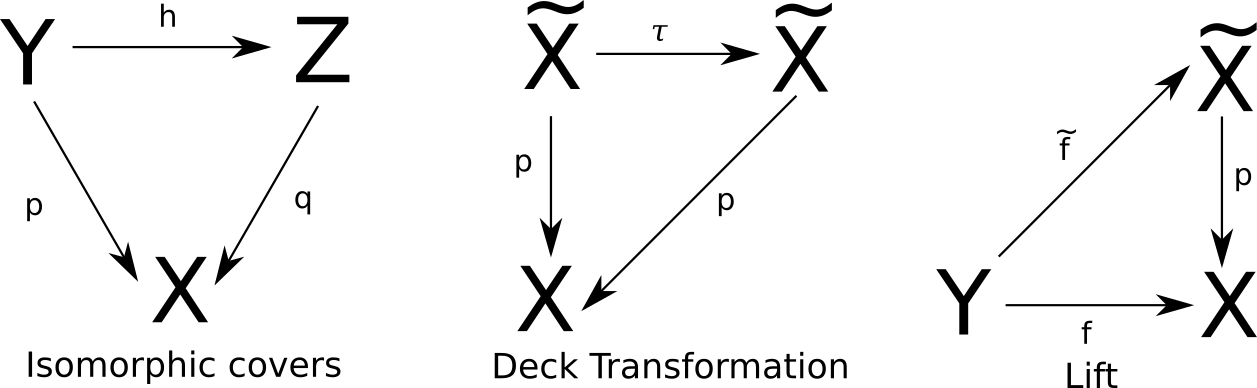
\includegraphics[width=4in]{basicdefs_diagrams.png}	
	\caption{Commutative diagrams defining various concepts}
\end{figure}

Here are some useful properties of lifts: 
\begin{enumerate}[label=(\roman*)]
	\item $\widetilde{f}:Y\to\widetilde{X}$ then $\widetilde{f}$ is a lift of $p\circ\widetilde{f}$.
	\item $\widetilde{f},\widetilde{g}:Y\to\widetilde{X}$ and $f\simeq g$ $\implies p\circ \widetilde{f}\simeq p\circ \widetilde{g}$ (homotopies descends).
	\item $\alpha, \beta: I \to \widetilde{X}$ such that $\alpha(1)=\beta(0)$ then $p\circ (\alpha\ast\beta)=(p\circ\alpha)\ast(p\circ\beta)$ (concatenation descends).
\end{enumerate}

\section{Homotopy Lifting Property}
\begin{defin}
	A map $p:Z\to X$ has the \mdf{homotopy lifting property} if given any homotopy $F:Y\times I \to X$ and any lift $g:Y\times\left\{0\right\}\to Z$ there exists a unique homotopy $\widetilde{F}:Y\times I \to Z$ satisfying
	\begin{enumerate}[label=(\roman*)]
		\item $\widetilde{f}_0=g$
		\item $p\circ\widetilde{F}=F$
	\end{enumerate}
	i.e. given a homotopy and a lift of one endpoint, there exists a unique lift of that homotopy.

	As a special case where $Y=\left\{pt\right\}$, a map $p:Z\to X$ has the \mdf{path lifting property} if for any path $f:I\to X$, $x_0\in X$ and $\widetilde{x}_0\in p^{-1}(x_0)$ there exists a unique path $\widetilde{f}:I\to Z$ such that 
	\begin{enumerate}[label=(\roman*)]
		\item $\widetilde{f}(0)=\widetilde{x}_0$
		\item $p\circ\widetilde{f}=f$
	\end{enumerate}
\end{defin}

\begin{lemma}[Local Homotopy Lifting Property]
Let $p:\widetilde{X}\to X$ be a covering map and $F:Y\times I \to X$ a homotopy.
Suppose we have $g:Y\times\left\{0\right\}\to \widetilde{X}$.
Then for every $y\in Y$
\begin{enumerate}[label=(\alph*)]
	\item There exists an open neighbourhood $N\subseteq Y$ and a unique homotopy $\widetilde{F}_N:N\times I \to \widetilde{X}$ such that
		\begin{enumerate}[label=(\roman*)]
			\item $(\widetilde{f}_N)_0=g$.
			\item $p\circ\widetilde{F}_N=\restr{F}{N\times I}$.
		\end{enumerate}
	\item If $M\subseteq Y$ with $y\in M$ is another open neighbourhood for which \textit{(a)} holds then \textit{(a)} also holds for $M\cap N$ and
		\[
			\restr{\widetilde{F}_N}{(M\cap N)\times I)}=\restr{\widetilde{F}_M}{(M\cap N)\times I}=\widetilde{F}_{M\cap N}
		\]
\end{enumerate}
\end{lemma}
\begin{proof}
This has a very long proof.
\end{proof}

\begin{prop}
Covering maps $p:\widetilde{X}\to X$ have the homotopy lifting property.
\end{prop}

\begin{proof}
Let $P;\widetilde{X}\to X$ be a covering map.
Let $F:Y\times I \to I$ be a homotopy and choose soma arbitrary starting $g:Y\times\left\{0\right\}\to\widetilde{X}$.

We can cover $Y=\cup_\alpha N_\alpha$ such that \textit{(a)} and \textit{(b)} hold from the lemma.

We can then define a new homotopy by stitching these together:
\[
	\widetilde{F}:Y\times I \to \widetilde{X},\quad\quad \widetilde{F}(y, t)\defeq \widetilde{F}_{N_\alpha}(y, t)\;\;\text{if}\;\; y\in N_\alpha
\]
We do not get any ambiguity here thanks to property \textit{(b)} from the lemma.
The continuity of this construction follows from the pasting lemma.
\end{proof}

\begin{theorem}
Let $\omega_n:I\to S^1$ be defined by $\omega_n(s)=e^{2\pi i n s}$. Then
\[
	\pi_1(S^1,1)=\left\{[\omega_n] \rmv n\in\Z\right\}
\]
\end{theorem}

\begin{proof}
Define $\Phi:\Z\to\pi_1(S^1,1)$ by $n\mapsto [\omega_n]$. We claim this is an isomorphism.
For this define the following useful maps
\begin{align*}
	p(t)&=e^{2\pi i t}	\\
	\omega_n(t) &= e^{2\pi i n t} \\
	\widetilde{\omega}_n(t) &= nt \\
	\tau_m(t)&=t+m
\end{align*}
\begin{itemize}
	\item \underline{$\Phi$ is a group homomorphism.}

		Then we can see that indeed $\widetilde{\omega_n}:\R\to\R$ is a lift of $\omega_n$.
		One can also see through the linear homotopy that
		\[
			\widetilde{\omega}_{m+n}\homrel \widetilde{\omega}_m\ast(\tau_m\circ \widetilde{\omega}_n)
		\]
		Now given any $m, n\in\Z$ we have
		\[
		\begin{WithArrows}
			\Phi(m+n) &= [\omega_{n+m}] \Arrow{\text{lift}}\\
					  &= [p\circ\widetilde{\omega}_{n+m}] \Arrow{\text{homotopies descend}}\\
					  &= \left[p \circ \left(\widetilde{\omega}_m\ast\left(\tau_m\circ\widetilde{\omega}_n\right)\right)\right] \\
					  &= [p\circ\widetilde{\omega_m}]\cdot[p\circ\tau_m\circ\widetilde{\omega}_n] \Arrow{\text{deck transformation}}\\
					  &= [p\circ\widetilde{\omega_m}]\cdot[p\circ\widetilde{\omega}_n]\Arrow{\text{lift}}\\
					  &= [\omega_m]\cdot[\omega_n]\\
					  &= \Phi(m)\cdot\Phi(n)
		\end{WithArrows}
		\]
	\item \underline{$\Phi$ is surjective.}

		Choose any $[\alpha]\in\pi_1(S^1,1)$, we aim to find $n\in\N$ such that $\alpha\homrel\omega_n$.
		We certainly know that $\alpha(0)=\alpha(1)=1$ and hence $p^{-1}(1)=\Z$ and in particular $0\in p^{-1}(1) = p^{-1}(\alpha(0))$.

		So by the path lifting property there exists a unique lift $\widetilde{\alpha}:I\to R$ such that 
		\begin{enumerate}[label=(\roman*)]
			\item $\widetilde{\alpha}(0)=0$.
			\item $p\circ\widetilde{\alpha}=\alpha$.
		\end{enumerate}
		Now, $\alpha(1)=1\implies p(\widetilde{\alpha}(1))=1 \implies \widetilde{\alpha}(1)\in p^{-1}(1)=\Z$.
		Suppose $\widetilde{\alpha}(1)=n\in\Z$.
		So $\widetilde{\alpha}$ is a path from $0$ to $n$ in $\R$.
		By the linear homotopy we can see that $\widetilde{\alpha}\homrel\widetilde{\omega}_n$.
		But homotopies descend and hence
		\[
			\alpha = p\circ \widetilde{\alpha}\homrel p\circ\widetilde{\omega}_n=\omega_n
		\]
	\item \underline{$\Phi$ is injective.}

		Assume that $\Phi(n)=[e]$.
		We aim to show that in fact $n=0$.

		To start, $\omega_n\homrel e$ and hence we have a homotopy $F:I\times I\to S^1,\;(s, t)\mapsto F(s, t)$ such that $f_0=\omega_n$, $f_1=e$ and $f_t(0)=f_t(1)=1$.

		Now by the HLP we see that there is a unique homotopy $F:I\times I \to R$ satisfying
		\begin{enumerate}[label=(\roman*)]
			\item $\widetilde{f}_0=\widetilde{\omega}_n$.
			\item $p\circ \widetilde{F}=F$.
		\end{enumerate}

		Now since the left, top and bottom edges were identically $1$ in $F$ we must have that the same edges lie in $\Z$ in the lifted homotopy.
		But consider the bottom edge $\widetilde{\omega}_n$.
		On the left side it is $0$ but on the right it is $n$.
		By continuity along the left, top and bottom edges of $\widetilde{F}$ we must have that $n=0$.
		This can be seen in Figure \ref{fig:circlepi1}.
		\begin{figure}[ht]
			\centering
			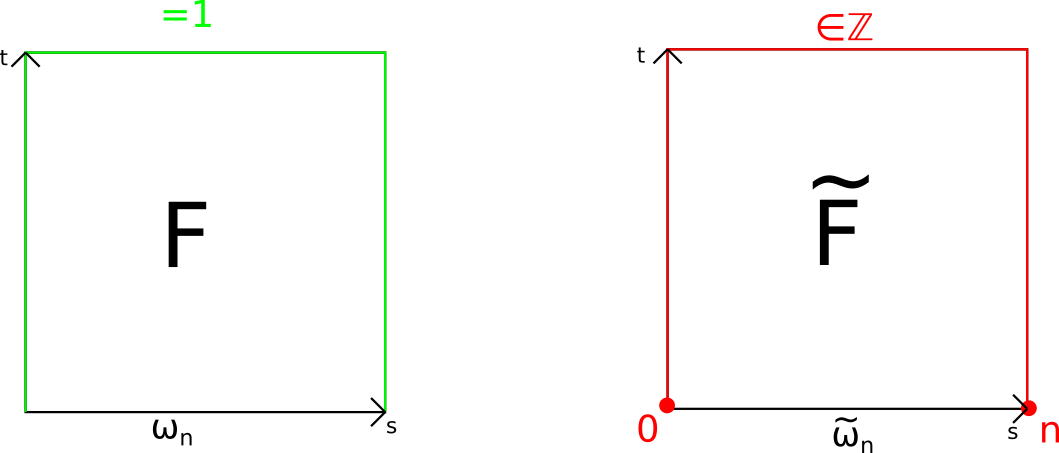
\includegraphics{circlepi1.png}
			\label{fig:circlepi1}
			\caption{Diagrammatic explanation of continuity argument}
		\end{figure}	
\end{itemize}
\end{proof}

\section{Applications}
\begin{defin}
	A \mdf{map of pairs} $f:(X,A)\to(Y, B)$ is a map $f:X\to Y$ such that $f(A)\subseteq B$.	

	The \mdf{induced homomorphism} of $f:(X, x_0)\to (Y, y_0)$ is the map
	\begin{align*}	
		f_\ast:\pi_1(X, x_0)&\to \pi_1(Y,y_0)\\
		[\alpha] &\mapsto [f \circ \alpha]
	\end{align*}
	We need to show that this is well-defined and is in fact a group homomorphism.
\end{defin}

\begin{lemma}[Functoriality]
$(g\circ f)_\ast = g_\ast \circ f_\ast$
\end{lemma}
\begin{cor}
If $f$ is a homeomorphism then $f_\ast$ is a group isomorphism.
\end{cor}
\begin{theorem}
let $f:X\to Y$ be a homotopy equivalence and $x_0\in X$.
Then $$f_\ast:\pi_1(X, x_0)\to\pi_1(Y, f(x_0))$$ is an isomorphism.
\end{theorem}

\begin{proof}
Let $y_0\defeq f(x_0)$ and $g:Y\to X$ be the homotopy inverse.
Denote $x_1\defeq g(y_0)$.
We get a homotopy a $K:X\times I \to X$ such that $k_0=id_X$ and $k_1=g\circ f$.

We define path in $X$ by following that path of $x_0$ under this homotopy, i.e.
\[
	h:I\to X\quad t\mapsto K(x_0, t)
\]
\textbf{Claim: }$\beta_h[\gamma]=(g\circ f)_\ast [\gamma]$ for all loops $\gamma$ based at $x_0$.

We have already seen that base point change homomorphisms are in fact isomorphisms and hence we have that $(g\circ f)_\ast = g_\ast \circ f_\ast$ is an isomorphism.
This implies that $g_\ast$ is surjective and $f_\ast$ is injective.
Repeating this argument with the other homotopy then yields the result.

\textbf{Proof of claim:}

Define a new homotopy by
\[
	H(s, t)\defeq
	\begin{cases}
		h(t) & \text{for } s\leq t \\
		h(s) & \text{for } s\geq t
	\end{cases}
\]
which has the properties that $h_0=h$ and $h_1=h(1)=x_1$.

Also define $K(\gamma(s), t)$ so that $\gamma_0=\gamma$ and $\gamma_1 = g\circ f \circ \gamma$.

Finally, one can check that $\alpha_t\defeq \overline{h_t}\ast \gamma_t\ast h_t$ gives a well-defined path for every $t$.
This gives a homotopy between
\begin{align*}
	\gamma_0&=\overline{h}\ast\gamma\ast h \quad\quad\quad\quad \text{and} \\
	\gamma_1&=e_{x_1}\ast(g\circ f\circ \gamma)\ast e_{x_1}
\end{align*}
\end{proof}

\begin{prop}
Consider the sequence of maps induced by a retract $r:X\to A$ and the `inverse' inclusion for a point $x_0\in A$
\[
	\pi_1(A,x_0)\xrightarrow{i_\ast}\pi_1(X, x_0)\xrightarrow{r_\ast}\pi_1(A, x_0)
\]
\begin{enumerate}
	\item $i_\ast$ is injective.
	\item $r_\ast$ is surjective.
	\item If $r\homrelset{A}id_X$ then the induced maps are in fact isomorphisms.
\end{enumerate}
\end{prop}
\begin{proof}
\textit{(1)} and \textit{(2)} follow immediately from the fact that $r\circ i = id_A$ and functoriality.

For \textit{(3)} it remains to show that $r_\ast$ is injective and $i_\ast$ is surjective.
For now we just show that $r_\ast$ is injective.
Suppose $r_\ast[\gamma]=[e]$ then we wish to show that in fact $[\gamma]=[e]$.

We know $r \circ \gamma \homrel e$ and $r \homrelset{A} id_X$.
We have a homotopy $F:X\times I \to X$ where $\restr{f_t}{A}=id_A$, $f_0=r$ and $f_1=id_X$.
We define a new homotopy $G:I\times I \to X$ by $G(x, t)= F(\gamma(x), t)$ which satisfies.
\begin{enumerate}[label=(\roman*)]
	\item $g_t(0)=g_t(1)=f_t(\gamma(0))=f_t(x_0)=x_0$ since $x_0\in A$.
	\item $g_0(x)=f_0(\gamma(x))=(r \circ \gamma)(x)$.
	\item $g_1(x)=f_1(\gamma(x))=\gamma(x)$.
\end{enumerate}
Hence we have $r\circ \gamma \homrel \gamma$ and hence $\gamma \homrel e$.
The proof that $i_\ast$ is surjective is very similar.
\end{proof}

\begin{theorem}[No Retract Theorem]
There is no retract $R:D^2\to S^1$.
\end{theorem}

\begin{proof}
Assume that such a retract exists then there is a surjective homomorphism $r_\ast$:
\[
	0=\pi_1(D^2,1)\to\pi_1(S^1,1)=\Z
\]
which is obviously nonsense.
\end{proof}

\begin{theorem}[Brouwer Fixed Point Theorem]
Any map $f:D^2\to D^2$ has a fixed point.
\end{theorem}

\begin{proof}
Assume that $f$ has no fixed point, then we construct the following map for every $x$ in $S^1$:
\[
	L_x(t)\defeq tx+(1-t)f(x)\quad \forall t\geq 0
\]
Then we can define a map $\phi:D^2\to S^1$ by
\[
	\phi(x)=L_x(\R_{\geq 0})\cap S^1
\]
which we claim is a retraction.
Certainly, $\restr{\phi}{S^1}=id_{S_1}$ but what about continuity?

Well $\phi(x)=L_x(t)$ for the unique $t$ which solves $\abs{L_x(t)}^2=1$ and is bigger than 0.
The equation for $t$ is quadratic and so $t$ can be shown to be a continuous function of $x$.
Then clearly $L_x$ is continuous so $phi$ is continuous.

The no retract theorem yields a contradiction.
\end{proof}
\begin{note}
The Brouwer Fixed Point Theorem also holds for sets $S\cong D^2$ and their boundary.
\end{note}
\subsection{Involutions and Borsuk-Ulam Theorem}
\begin{defin}
	Given a topological space $X$, an \mdf{involution} is a map $h:X\to X$ such that for every $x\in X$
	\[
		h(h(x))=x.
	\]
	We often write h(x)=-x for convenience.

	Given spaces $X$ and $Y$ each with involutions and a map $f:X\to Y$, we say f is
	\begin{align*}
		\mdf{\text{odd}}\quad&\text{if}\quad f(-x)=-f(x) \\
		\mdf{\text{even}}\quad&\text{if}\quad f(-x)=f(x)
	\end{align*}
	for all $x$ in $X$.

	A map $f:(X,x_0)\to (Y,y_0$ is \mdf{null-homotopic} if $f$ is homotopic to a constant map.

	A map $f:(X,x_0)\to (Y,y_0)$ is \mdf{null-homotopic relative to base points} if there is a homotopy between $F:X\times I \to Y$ such that $f_0=f$, $f_1=e_{y_0}$ and $f_t(x_0)=y_0$ for all $t$.
	We then write $f\homrelset{x_o} e_{y_0}$.
\end{defin}
\begin{prop}
If $f:S^1 \to S^1$ is odd then $f$ is not null-homotopic.
\end{prop}
\begin{proof}
Assume that $f$ is odd and null-homotopic to a constant path.
Without loss of generality we can assume that this constant path is at $1\in S^1$ because the space is path connected.
Label this homotopy $F:S^1\times I \to S^1$.
Consider the usual cover $p:\R\to S^1$.
We proceed by two steps
\begin{enumerate}
	\item \textbf{Use the oddity of $f$ to construct a loop in $S^1$ that lifts to a path from $0$ to $2n+1$}

		Define the map $\gamma:I \to S^1$ by  
		\[
			\gamma(t)=\frac{f(q(t))}{f(1)}
		\]
		where $q$ is the quotient map $[0,1]\to S^1$ or $q(t)=e^{2\pi i t}$.
		Thanks to the oddity of $f$ we get the property that
		$\gamma(s+\frac{1}{2})=-\gamma(s)$ for all $s\in[0 , \frac{1}{2}]$.
		Note also that $\gamma(0)=\gamma(1)=1$ and hence $\gamma(\frac{1}{2})=-1$.

		Now apply the path-lifting property of $p$ to $\gamma$ to get a curve $\widetilde{\gamma}:I\to \R$  such that $\widetilde{\gamma}(0)=0$.
		Then $\widetilde{\gamma}(\frac{1}{2})=n+\frac{1}{2}$ for some $n\in\Z$.
		Our aim now is to show that $\widetilde{\gamma}(1)=2n+1$.

		We can consider the following two paths.
		$\alpha$ represents what we thing $\widetilde{\gamma}$ does on the second half and $\beta$ is what $\widetilde{\gamma}$ actually does
		\[
			\alpha(s)\defeq n+\frac{1}{2}+\widetilde{\gamma}\left(\frac{s}{2}\right)
		\quad\quad	\beta (s)\defeq \widetilde{\gamma}\left(\frac{s+1}{2}\right)
		\]
		Then
		\begin{itemize}
			\item $p\circ\alpha(s)=-\gamma(\frac{s}{2})=\gamma(\frac{s}{2}+\frac{1}{2})=p\circ\beta(s)$
			\item $\alpha(0)=\beta(0)=n+\frac{1}{2}$
		\end{itemize}
		So by the uniqueness of lifts its follows that
		\[
			2n+1 = \alpha(1) = \beta(1) = \widetilde{\gamma}(1)
		\]
	
	\item \textbf{Get a contradiction by showing $\widetilde{\gamma}\simeq e$ and hence $2n+1 = 0$}

		We known that $F$ is a homotopy between $f$ and a constant map $S^1\to S^1$.
		So we can construct a homotopy from $\gamma$ to a constant path by
		\[
			\Gamma:I \times I \to S^1 \quad (s, t)\mapsto \frac{F(e^{2\pi i s}, t)}{F(1, t)}
		\]
		where we use complex number division.
		We see that this is $\gamma$ on the bottom and $1$ on the other boundaries and hence the HLP yields a homotopy with $\widetilde{\gamma}$ on the bottom.
		The boundaries go to a constant path and hence $0=2n+1$.
		This is clearly a contradiction so $f$ was not null-homotopic.
		\begin{figure}[ht]
			\centering
			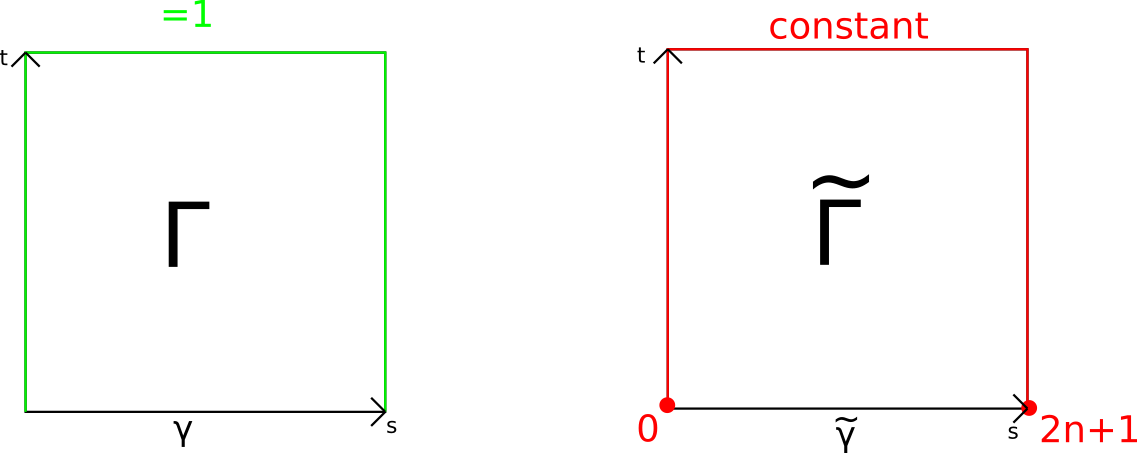
\includegraphics[width=4in]{odd-null.png}
			\caption{Explaining why $0=2n+1$}
		\end{figure}
		
\end{enumerate}

\end{proof}

\begin{cor}
	If $f:S^2 \to \R^2$ is odd then there is a point $x\in S^2$ such that $f(x)=0$.
\end{cor}

\begin{proof}
Assume that $f$ is odd and non-vanishing for all $x\in S^2$.
We're going to define maps $g,p$ that together form a homotopy from an odd map to a constant path
\begin{figure}[H]
	\centering
	\begin{tikzcd}
		S^1 \times I \arrow[rr, "H"] \arrow[rd, "p"'] & \; & S^1 \\
		\; & S^2 \arrow[ru, "g"']
	\end{tikzcd}
\end{figure}
We can now define the maps
\[
	g:S^2\to S^1 \quad \quad g(x)\defeq\frac{f(x)}{\norm{f(x)}}
\]
Note that $g$ is odd.
Let $U$ denote the upper hemi-sphere of $S^2$ then we can define $p:S^1\times I \to U$ by
\[
	p(e^{i\theta}, t) \defeq (t\cos(\theta), t\sin(\theta), \sqrt{1-t^2})
\]
Note that $p_0$ is constant and $p_1$ embeds $S^1$ into the equator.
Finally we construct a homotopy $H\defeq g \circ p$.
Notice that $h_0=g\circ p_0$ which is constant where as $h_1=g\circ p_1$ is an odd map since $g$ and $p_1$ are both odd.
\end{proof}

\begin{theorem}[Borsuk-Ulam]
Given a map $f:S^2\to\R^2$ there is a point $x\in S^2$ such that $f(-x)=f(x)$.
\end{theorem}
\begin{proof}
The map $g(x)\defeq f(x) - f(-x)$ is by construction odd and hence has a vanishing point.
\end{proof}

\section{Product Spaces}
Given pointed spaces $(X, x_0)$ and $(Y, y_0$ then
\[
	\pi_1(X\times Y, (x_0, y_0))\cong \pi_1(X, x_0)\times\pi_1(Y,y_0)
\]
Also homotopies of paths in $X\times Y$ correspond to pairs of homotopies in $X$ and $Y$.

\subsection{Fundamental group of $S^n$ for $n\geq 2$}
\begin{theorem}
For all $n\geq 2$ the fundamental group of $S^n$ is trivial.
\end{theorem}
\textbf{Idea: }Use stereographic projection into $\R^n$ and then use the linear homotopy.

The main issue with this is that the loop may go around or through the north pole, at which point our projection breaks down.
However, in these big spheres we should be able to find a point that isn't inside the loop and project from there.
Note that in $S^1$ we cannot do this because every non-trivial curve uses every point.
\begin{proof}
Cover the sphere with two open sets such that $U_1, U_2$ such that $x_0\in U_1\cap U_2$ and $U_1\cap U_2$ is path connected.
Now take any loop $\gamma:I\to S^n$ and subdivide the interval as
\[
0= t_0 < t_1 < \dots < t_m = 1
\]
such that for all $i$ there is a $j$ such that $\gamma[t_{i-1}, t_i]\subseteq U_j$.
So we can now view $\gamma$ is the concatenation
\[
	\gamma=\bigast_{i-1}^m \restr{\gamma}{[t_{i-1}, t_i]}
\]
Now since $x_0$ and $\gamma(t_i)$ are both in $U_1\cap U_2$, we can let $\alpha_i$ be a path in $U_1\cap U_2$ from $\gamma(t_i)$ to $x_0$.
Now we can put these paths in between the subdivisions of $\gamma$:
\[
	\beta\defeq \left[\restr{\gamma}{[t_0, t_1]}\ast\alpha_1\right]\ast\left[\bigast_{i=2}^{m-1} \overline{\alpha}_{i-1}\ast\restr{\gamma}{[t_{i-1}, t_i]}\ast \alpha_i\right]\ast \left[\overline{\alpha}_{m-1}\ast\restr{\gamma}{[t_{m-1}, t_m]}\right]
\]
Now each $\overline{\alpha}_{i-1}\ast\restr{\gamma}{[t_{i-1}, t_i]}\ast\alpha_i$ lies in one $U_j$ and so is homotopic to a constant loop by using the linear homotopy in $\R^n$.
So $\beta\simeq e_{x_0}$ and $\beta\simeq\gamma$ and hence $\gamma\simeq e_{x_0}$.
\end{proof}

\section{Some Algebra}
\begin{prop}
Let $p:\widetilde{X}\to X$ be a covering , $x_0\in X$ and $\widetilde{x}_0\in p^{-1}(x_0)$.
\begin{enumerate}
	\item The induced map $p_\ast:\pi_1(\widetilde{X}, \widetilde{x}_0)\to \pi_1(X, x_0)$ is injective.
	\item If $[\alpha]\in\pi_1(X, x_0)$ and $\widetilde{\alpha}$ is a lift of $\alpha$ such that $\widetilde{\alpha}(0)=\widetilde{x}_0$, then
		\[
			[\alpha]\in p_\ast(\pi_1(\widetilde{X}, \widetilde{x}_0)) \iff \widetilde{\alpha}\text{ is a loop}
		\]
\end{enumerate}
\end{prop}
\begin{proof}
\begin{enumerate}
	\item We wish to show that $p_\ast([\widetilde{\alpha}])=[p\circ \widetilde{\alpha}]=[e_{x_0}]\implies [\widetilde{\alpha}]=[e_{\widetilde{x}_0}]$.

	Given $[\widetilde{\alpha}]\in\pi_1(\widetilde{X}, \widetilde{x}_0)$ such that $[p\circ\widetilde{\alpha}]=[e_{x_0}]$, define $\alpha\defeq p\circ\widetilde{\alpha}$ and then $\widetilde{\alpha}$ is the unique lift of $\alpha$ with the property $\widetilde{\alpha}(0)=\widetilde{x}_0$. 
	Now, by assumption, $\alpha\homrel e_{x_0}$ and hence there is a homotopy $F:I\times I \to X$ with $f_0=\alpha$, $f_1=e_{x_0}$.

	By the HLP, there exists a unique lift $\widetilde{F}:I\times I \to X$ such that $\widetilde{f}_0=\widetilde{\alpha}$.
	Now $F(0, t)$, $F(1, t)$ and $F(s, 1)$ are all constant paths at $x_0$ and hence lift to constant paths at $\widetilde{x}_0$.
	So $\widetilde{F}$ tells us that $\widetilde{\alpha}\homrel e_{\widetilde{x}_0}$.

	\item We really only have the forward direction to prove.

		Suppose $[\alpha]\in p_\ast(\pi_1(\widetilde{X}, \widetilde{x}_0))$ then $[\alpha]=[p\circ \widetilde{\gamma}]$ for some $[\widetilde{\gamma}]\in\pi_1(\widetilde{X}, \widetilde{x}_0)$.
		Suppose $\widetilde{\alpha}$ is a lift of $\alpha$ with $\widetilde{\alpha}(0)=\widetilde{x}_0$.
		We have
		\[
			\alpha = p\circ \widetilde{\alpha}\homrel p\circ\widetilde{\gamma}\eqdef\gamma
		\]
		We can lift the homotopy to one in $\widetilde{X}$ that starts at $\widetilde{\alpha}$.
		Then the top of the new homotopy must be a lift of $\gamma$ which starts at $\widetilde{x}_0$ (since the left hand side of $\widetilde{F}$ is constant and starts at $\widetilde{x}_0$).
		By the Path Lifting Property, $\widetilde{\gamma}$ is the unique path with these properties.
		So we can lift the homotopy between $\alpha$ and $\gamma$ to one between $\widetilde{\alpha}$ and $\widetilde{\gamma}$.
		The right hand side of $\widetilde{F}$ must then be a constant path at $\widetilde{x}_0$ proving the claim.
		
		\begin{figure}[ht]
			\centering
			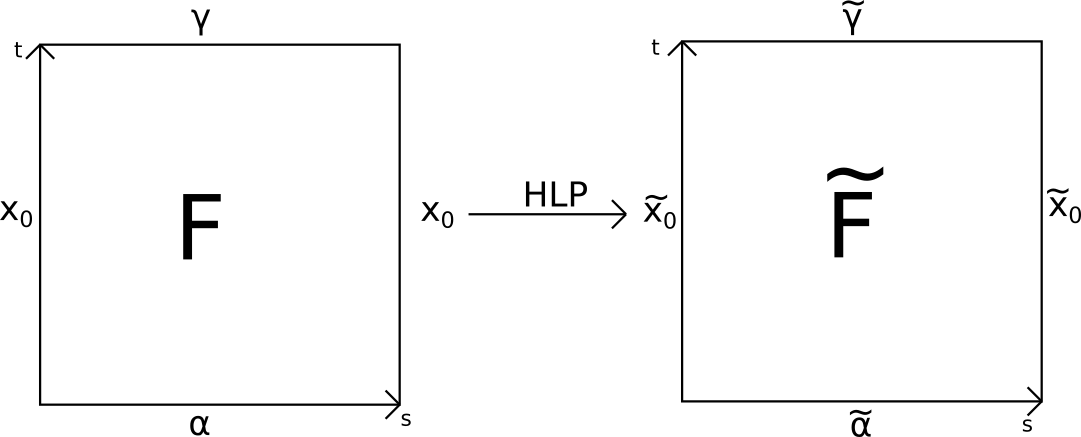
\includegraphics[width=4in]{HLPdiagram_1.png}
			\caption{Diagrammatic explanation that $\widetilde{\alpha}$ is a loop at $\widetilde{x}_0$.}
		\end{figure}
\end{enumerate}
\end{proof}

\begin{defin}
Given a group $G$ and a subgroup $H\leq G$ we have the \mdf{quotient space}
\[
	\frac{G}{H}\defeq\left\{Hg \rmv g\in G\right\} = \left\{\text{right cosets}\right\}
\]
and then the \mdf{index} is $[G:H]=\abs{\frac{G}{H}}=\#\text{ of cosets}$.

Let $p:\widetilde{X}\to X$ be a cover and assume that both spaces are path connected.
Then we define the \mdf{degree} 
\[
	\deg(p)=\abs{p^{-1}(x)} \quad\text{for any}\quad x\in X
\]
\end{defin}
\begin{note}
	Definition of cover $\implies$ $\deg(p)$ is at least locally constant.

	Path connected $\implies$ globally constant.
\end{note}
\begin{prop}
Let $p:\widetilde{X}\to X$ be a cover with $\widetilde{X}, X$ path connected, $x_0\in X$ and $\widetilde{x}_0\in p^{-1}(x_0)$.
Then \[
	\deg(p)\defeq\left[\pi_1(X, x_0) : p_\ast(\pi_1(\widetilde{X}, \widetilde{x}_0))\right].
\]
\end{prop}
\begin{proof}

Let $G\defeq\pi_1(X,x_0)$ and $H\defeq p_\ast(\pi_1(\widetilde{X}, \widetilde{x}_0))$.
Given any $[\alpha]\in G$ we get a unique lift $\widetilde{\alpha}$ with $\widetilde{\alpha}(0)=\widetilde{x}_0$ and then $\widetilde{\alpha}(1)=\widetilde{x}_1\in p^{-1}(x_0)$.

Now let $[\gamma]\in H$ then we have
\begin{align*}
	\begin{WithArrows}
		[\gamma]\in H &\implies [\gamma]\cdot [\alpha] = [\gamma \ast \alpha]\in H [\alpha]\\
					  &\implies \widetilde{\gamma}\text{ (a lift of }\gamma\text{) is a loop at }\widetilde{x}_0 \Arrow{unique lift} \\
					  & \implies (\gamma\ast\alpha) \text{ lifts to }(\widetilde{\gamma}\ast\widetilde{\alpha})\text{ from }\widetilde{x}_0\text{ to }\widetilde{x}_1
	\end{WithArrows}
\end{align*}

And hence we can construct a map
\[
	\Phi:\frac{G}{H}\to p^{-1}(x_0), \quad H[\alpha]\mapsto\widetilde{\alpha}(1)
\]
which we just showed is independent of the representative of $H[\alpha]$.
We wish to show that $\Phi$ is bijective.

\textbf{Injective: }Assume that $\Phi(H[\alpha])=\Phi(H[\beta])$ then $\widetilde{\alpha}(1)=\widetilde{\beta}(1)$.
Write $\gamma\defeq\alpha\ast\overline{\beta}$ then $\widetilde{\gamma}=\widetilde{\alpha}\ast\widetilde{\beta}$ is a loop because
$\widetilde{\alpha}(0)=\widetilde{\beta}(0)=\widetilde{\overline{\beta}}(1)=\widetilde{x}_0$ and the assumption means that $\widetilde{\alpha}$ and $\widetilde{\beta}$ join up in the middle.

Hence $[\gamma]=[\alpha]\cdot[\beta]^{-1}\in H$ so $H[\alpha]=H[\beta]$.

\textbf{Surjective: }This follow from path connectivity.
\end{proof}

\begin{defin}
	Let $\left\{X_\alpha, x_\alpha\right\}$ be a collection of pointed topological spaces.
	The \mdf{wedge product} is then defined to be
	\[
\bigvee_\alpha X_\alpha=\bigsqcup_\alpha \frac{X_\alpha}{x_\alpha\sim x_\beta}
	\]

	Then $\left\{G_\alpha\right\}_\alpha$ be some groups.
	Then a \mdf{word} on $\left\{G_\alpha\right\}_\alpha$ is a finite sequence
	\[
g = g_1 \dots g_m 
	\]
	for some $g_i \in G_{\alpha_i}$.
	Then $m$ is the \mdf{length} of the word $g$.

	We can concatenate words $g=g_1, \dots, g_m$ and $h=h_1, \dots, h_n$ by
	\[
		g\ast h = g_1\dots g_m h_1 \dots h_n
	\]

	A word is said to be \mdf{reduced} if
	\begin{enumerate}[label=(\alph*)]
		\item $g_i\neq e_{\alpha_i}\quad\forall i$
		\item $\alpha_i\neq\alpha_{i+1}\quad\forall i$
	\end{enumerate}

	We can define the set
	\[
		\bigast_\alpha G_\alpha \defeq\left\{\text{reduced words on} \left\{G_\alpha\right\}_\alpha\right\}
	\]
	which we can given a product in the following way.
	Given $g,h\in\ast_\alpha G_\alpha$
	\begin{enumerate}
		\item Take the concatenation $g\ast h=g_1\dots g_m h_1 \dots h_n$.
		\item If $g_m$ and $h_1$ lie in different $G_\alpha$ then $g\cdot h \defeq g\ast h$.
		\item Else replace $g_m h_1$ by the product.
		\item If $g_m h_1=e$ then remove it and repeat from step 1 with the word $g_1\dots g_{m-1} h_2 \dots h_n$.
	\end{enumerate}
\end{defin}

\begin{theorem}
So defined, $(\ast_\alpha G_\alpha, \cdot)$ forms a group, called the \mdf{free product} of $\left\{G_\alpha\right\}_\alpha$.
\end{theorem}

\begin{proof}
The only difficult part is associativity, worth reading up on.
\end{proof}

\begin{lemma}
Let $\left\{\phi_\alpha: G_\alpha\to G \right\}_\alpha$ be a collection of group homomorphisms.
Then $\exists !$ group homomorphism $\ast_\alpha \phi_\alpha: G_\alpha \to G$ such that $\left(\ast_\alpha\phi_\alpha\right)\circ i_\alpha = \phi_\alpha \quad \forall \alpha$
\end{lemma}

\begin{proof}
Really the only thing to prove is that this definition doesn't depend on how the word is reduced.
\end{proof}

\begin{figure}[H]
	\centering
	\begin{tikzcd}
	& \pi_1(A_\alpha, x_0) \arrow[rrd, "(i_\alpha)_\ast", bend left=15] \arrow[rd] \\
	\pi_1(A_\alpha \cap A_\beta, x_0)\arrow[ru, "(i_{\alpha\beta})_\ast"] \arrow[rd, "(i_{\beta\alpha})_\ast"']& \; &
	\ast_\alpha \pi_1(A_\alpha, x_0) \arrow[r, dashed, "\Phi"] &
	\pi_1(X, x_0) \\
	& \pi_1(A_\beta, x_0) \arrow[ru] \arrow[rru, "(i_\beta)_\ast"', bend right =15]
	\end{tikzcd}
	\caption{The holy commutative diagram}
\end{figure}

\begin{theorem}[Seifert-van Kampen]
Let $X=\cup_\alpha A_\alpha$ be an open cover with $x_0\in\cap_\alpha A_\alpha$, then
\begin{enumerate}[label=(\roman*)]
	\item If $A_\alpha\cap A_\beta$ is path connected for all $\alpha, \beta$ then the induced map
		\[
			\Phi\defeq\bigast_\alpha(i_\alpha)_\ast:\bigast_\alpha \pi_1(A_\alpha, x_0) \to \pi_1(X, x_0)
		\]
		is surjective
	\item If $A_\alpha \cap A_\beta \cap A_\gamma$ is path connected for all $\alpha, \beta, \gamma$ then
		\[
			\ker(\Phi)=N=\langle\langle\left\{(i_{\alpha\beta})_\ast(\omega)\cdot(i_{\beta\alpha})_\ast(\omega)^{-1} \rmv \omega\in\pi_1(A_\alpha\cap A_\beta, x_0)\text{ for some }\alpha,\beta\right\}\rangle\rangle
		\]
		and hence 
		\[
			\pi_1(X, x_0)\cong \frac{\bigast_\alpha \pi_1(A_\alpha, x_0)}{N}
		\]
\end{enumerate}
\end{theorem}

\begin{lemma}
If $X=\cup_\alpha A_\alpha$ is an open cover with $A_\alpha \cap A_\beta$ path connected for every pair $\alpha, \beta$ and $x_0\in\cap_\alpha A_\alpha$, then every loop $\gamma$ based at $x_0$ in $X$ factors as
\[
[\gamma]=[\gamma_1]\cdot[\gamma_2]\cdot\dots\cdot[\gamma_m]
\]
with each $\gamma_i$ being a loop in $A_{\alpha_i}$.
\end{lemma}

\begin{proof}
Note than we can cover $I$ by the $\gamma^{-1}(A_\alpha)$ and since $I$ is compact we can actually reduce this to a finite sub cover.
Then the Lebesgue covering lemma means that we can find
\[
0=t_0 < t_1 < \dots < t_m = 1
\]
such that $\gamma[t_i, t_{i+1}]\subseteq A_{\alpha_{i+1}}$ for each $i\in[0, m)$.
Then for each $t_i$ notice that $\gamma(t_i)\in A_{\alpha_i}\cap A_{\alpha_{i+1}}$ which is path connected and hence there is a path $g_i$ from $\gamma(t_i)$ to $x_0$ in $A_{\alpha_i}\cap A_{\alpha_{i+1}}$.


Now we can define a new path $\hat{\gamma}$ by going back to $x_0$ along these paths at each $t_i$ and then returning to continue the loop.
Since $g\ast\overline{g}$ is homotopic to $e_{\gamma(t_i)}$ we have that $\hat{\gamma}\homrel\gamma$ and hence we can decompose $\gamma$ as required.
\end{proof}

These essentially proves part \textit{(i)} of the Seifert-van Kampen theorem.

\begin{defin}
	A \mdf{factorisation} of $[f]\in\pi_1(X, x_0$ is a sequence
	\[
		[f_1], \dots, [f_m] \quad \text{with}\quad [f_i]\in\pi_1(A_{\alpha_i}, x_0)
	\]
	such that $f\simeq f_1\ast \dots f_m$ (although this is not necessarily in reduced form).

	If $[f_i], [f_{i+1}]\in\pi_1(A_\alpha, x_0)$ then a \mdf{reduction} is
	\[
		[f_1] \dots [f_m] \mapsto [f+1] \dots [f_i \ast f_{i+1}] \dots [f_m] 
	\]
	(or an \mdf{expansion} if you go in the opposite direction).

	If $[f_i]=(i_{\alpha\beta})_\ast(\omega)$ and $[g_i]=(i_{\beta\alpha})_\ast(\omega)$ for some $\omega\in\pi_1(A_\alpha\cap A_\beta, x_0)$ then an \mdf{exchange} is
	\[
		[f_1]\dots[f_i]\dots[f_m]\mapsto [f_1]\dots[g_i]\dots[f_m]
	\]

	Two factorisations of $f$ are said to be \mdf{equivalent} if tone can be transformed to the other by a sequence of the above operations.
\end{defin}

\begin{lemma}
Under the conditions of Seifert-van Kampen \textit{(ii)} any two factorisations of $f$ are equivalent.
\end{lemma}

\begin{proof}
In lecture notes.
\end{proof}

This can then be used to proved Siefert-can Kampen \textit{(ii)}.

\section{CW Complexes}
\begin{defin}
	Given a space $X$ we can build up the \mdf{CW complex} recursively as follows:
	\begin{enumerate}
		\item $X_0$ is a discrete set called the \mdf{$0$-skeleton}.
		\item Given $X^{n-1}$ and a collection of \mdf{$n$-cells} $\left\{D_\alpha^n\right\}_\alpha$ and attaching maps $\phi_\alpha:\partial D_\alpha^n\to X^{n-1}$ we subsequently define $X_n$ by
			\[
				X^n\defeq\frac{\left[X^{n-1}\sqcup\left(\bigsqcup_\alpha D_\alpha^n \right)\right]}{x\sim \phi_\alpha(x)}
			\]
		\item Then $X=\cup_n X^n$, bestowed with the \mdf{weak topology} is a \mdf{CW complex}.
	\end{enumerate}


	Then X is called \mdf{finite dimensional} if $X=X^n$ for some $n\in\N$.

	Lastly, $X$ is \mdf{finite} if $\left\{D_\alpha^n \right\}_{\alpha, n}$ is finite (i.e. it is composed of finitely many cells).

	A \mdf{subcomplex} of $X$ is the closure in $X$ of a collection of open cells in $X$.
\end{defin}
\begin{note}
		$U\subseteq X \text{ is open in the weak topology} \iff \forall n \quad U\cap X^n \text{ is open in } X^n$
\end{note}

\subsection{Examples}

\subsubsection{M\"obius Strip}
The M\"obius strip $M$ can be defined as $I\times I$ after identifying $(0, x)$ with $(1, 1-x)$ for all $x\in I$.

One can give the M\"obius strip a CW structure by taking two 0 cells for either side of the identified line, three 1 cells (one for the identified line and two for the remaining boundaries) and then gluing a rectangle along the inside in the natural way.
Note that the M\"obius strip has a circle at its centre and the strip deformation retracts to it by taking the obvious retract on $I\times I $ and then passing to the quotient.
Hence $\pi_1(M)\cong\Z$.
Notes, the M\"obius strip has exactly one circle at its boundary.

\subsubsection{Real projective space}
Recall that we define real projective space $\RP^n$ by
\[
	\RP^n\defeq\frac{S^n}{x\sim -x}
\]
identifying antipodal points on the $n$-sphere.
Let $q$ be the quotient map from this definition.
We can define a CW structure on $\RP^n$ recursively as follows.

Consider the open set $U_0\defeq\left\{\left[(x_0, x_1, \dots, x_n\right] \rmv x_0 \neq 0\right\}$.
Then $\RP^n\setminus U_0=\left\{\left[0, x_1, \dots, x_n\right]\right\}$ is naturally homeomorphic to $\RP^{n-1}$.
Moreover, since $q$ is a two-sheeted covering we see that $q^{-1}(U_0)$ consists of the disjoint union of the sets $\left\{x_0 < 0\right\}$ and $\left\{x_0 >0\right\}$.
Each of these sets is the interior of an $n$-balls and maps homeomorphically to $U_0$ and hence $U_0\cong e^n$.

Set $D^n=\left\{x_0 \geq 0\right\}$ and $S^{n-1}=\partial D^n=\left\{(0, x_1, \dots , x_n)\right\}$ so we get the two-fold covering
\[
	\phi:S^{n-1}\to\RP^{n-1}
\]
which we can use as the attacking map to glue $D^n$ onto $RP^{n-1}$ where we removed $U_0$ and hence
\[
	\RP^n=\RP^{n-1}\sqcup\frac{D^n}{x\sim \phi(x)}
\]
Once can continue this process on iteratively and each stage we add one extra $n$-cell and hence
\[
	\RP^n=\left\{pt\right\}\cup e^1 \cup e^2 \cup \dots \cup e^n
\]

\textbf{n=0:} $\RP^0=\left\{pt\right\}$ so there is not much to say here.

\textbf{n=1: }$\RP^1=\RP^0\sqcup \frac{D^1}{0\sim 1}$ which show that $\RP^1$ is just a circle.

\textbf{n=2: }We attach a $2$-cell by gluing the boundary of a disk $D^2$ to $\RP^1$ by the usual two fold covering $S^1\to\RP^1$.
Perhaps a better way of thinking about $\RP^2$ is to start with the closed upper hemisphere.
Each point corresponds to a unique point in $\RP^2$ except at the boundary where we identify antipodal points.
So the boundary becomes a copy of $\RP^1$.

\begin{figure}[ht]
	\centering
	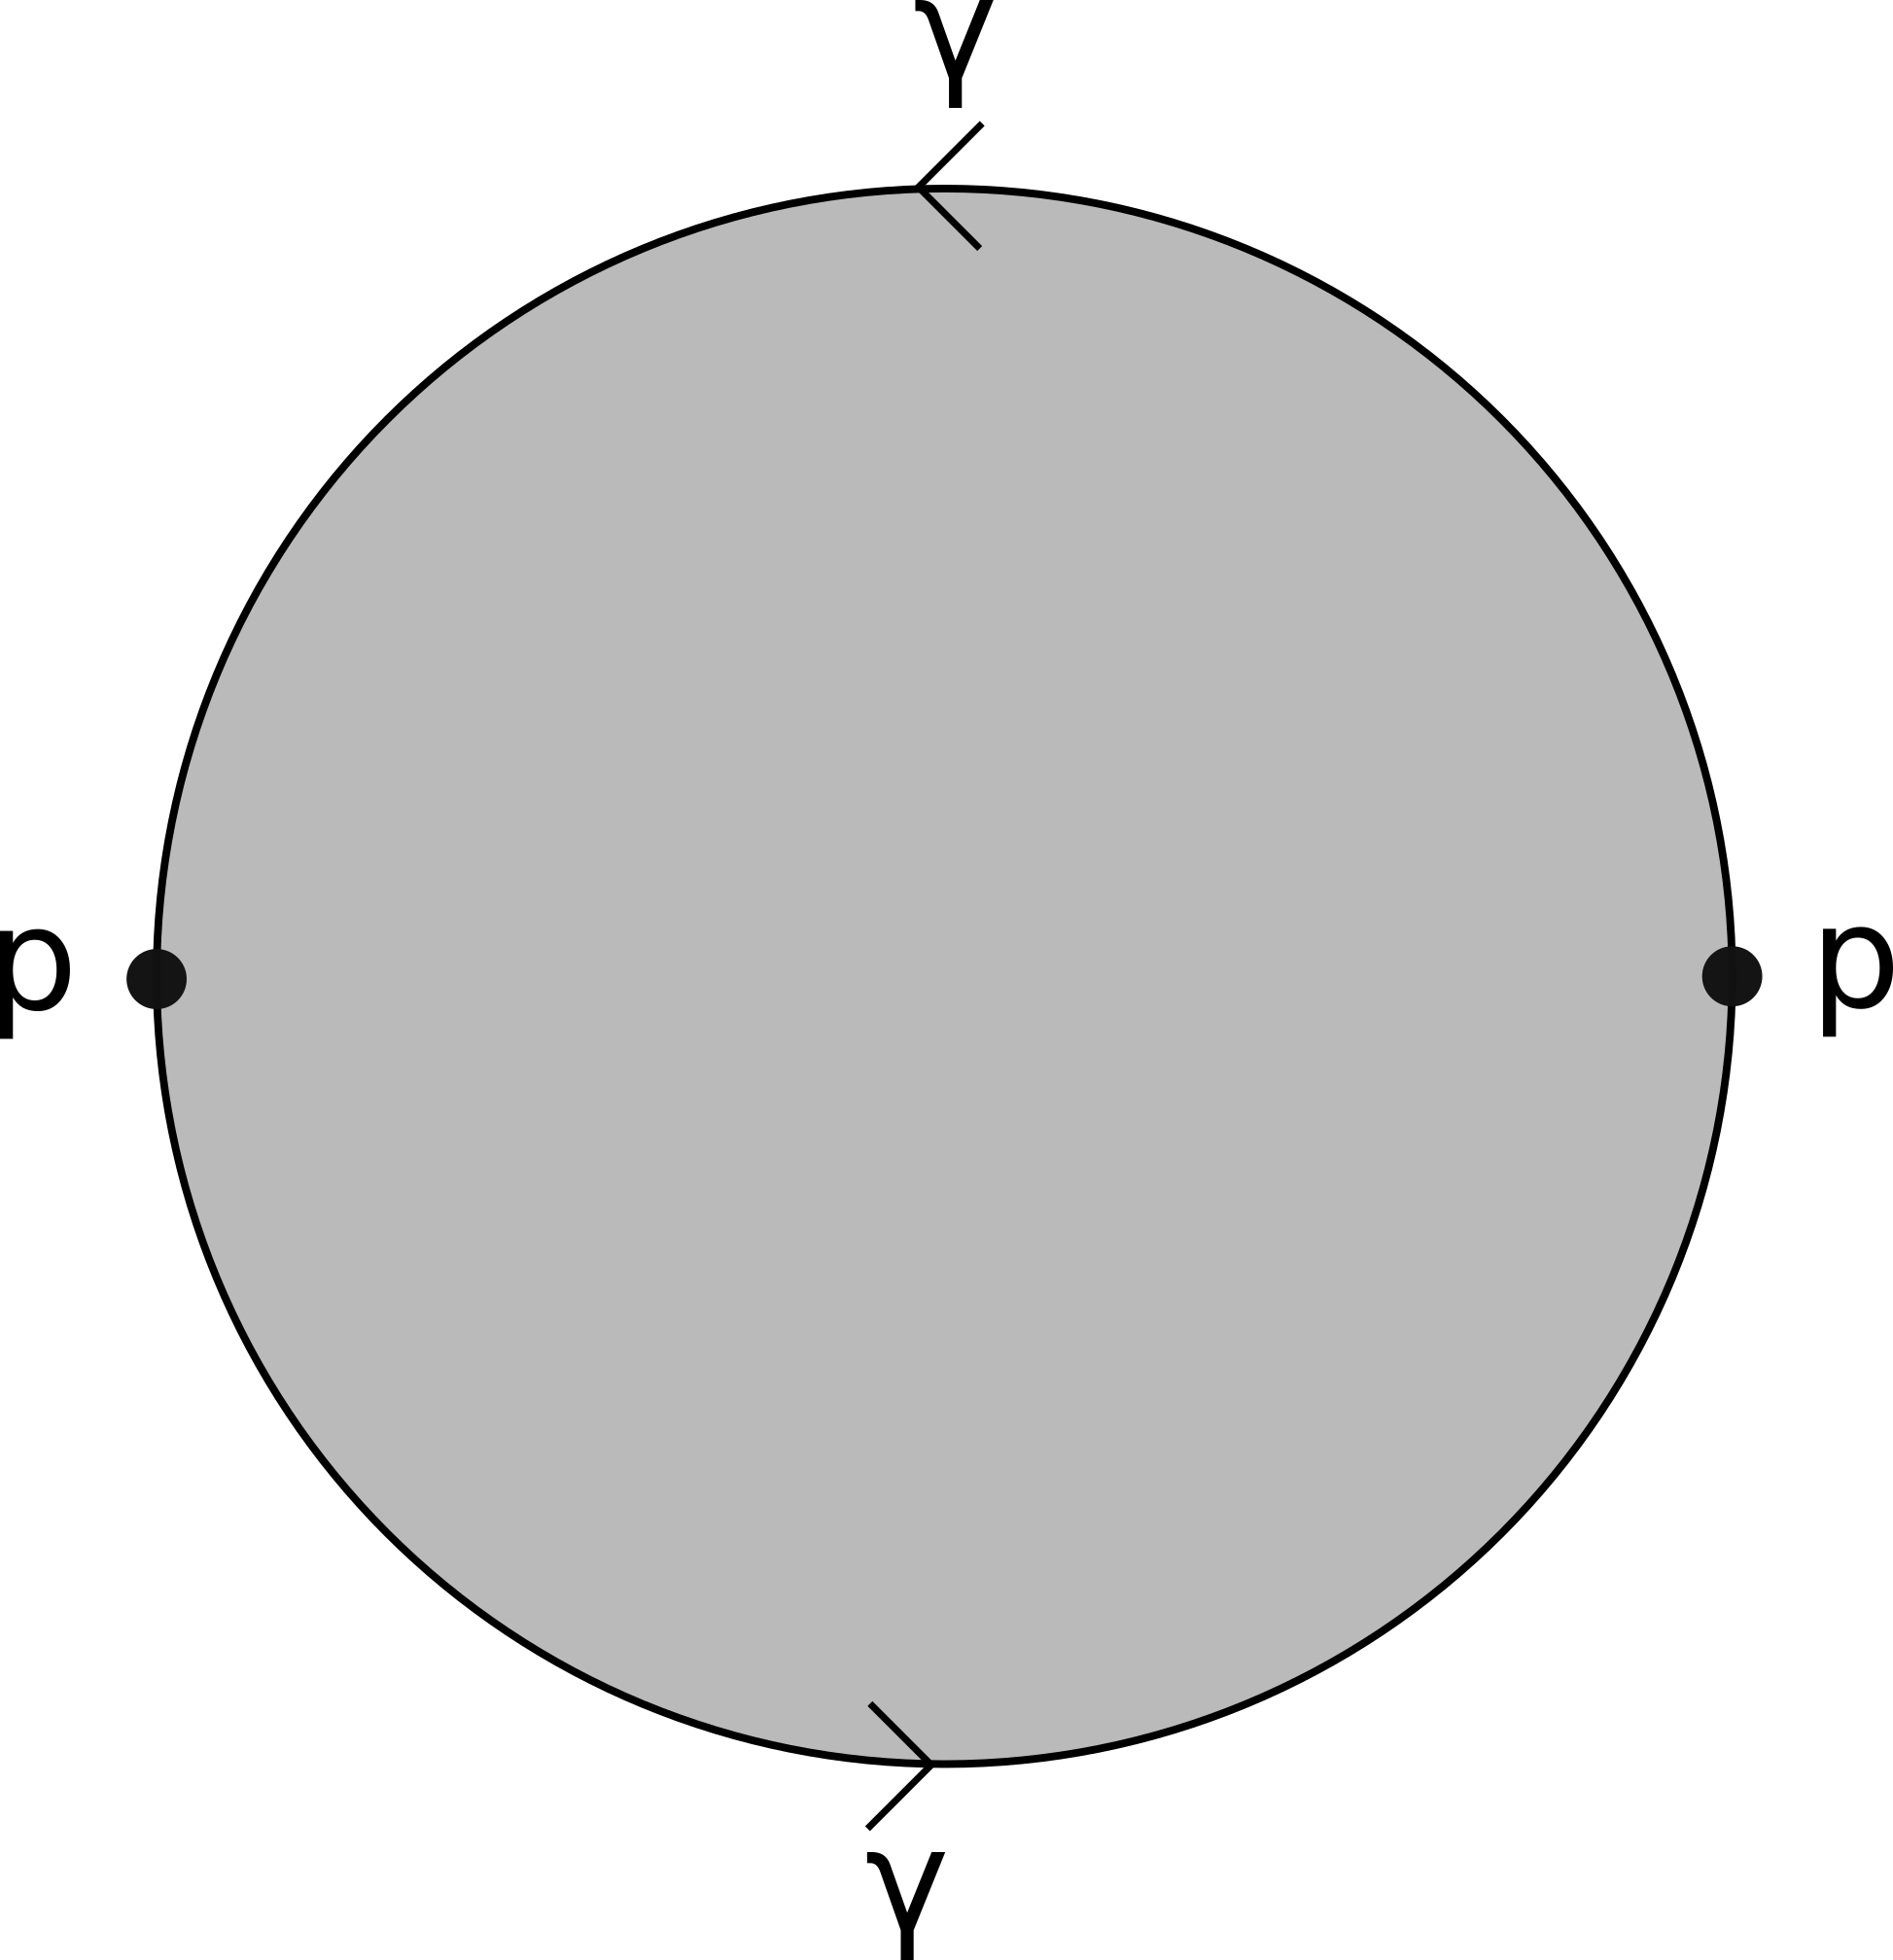
\includegraphics[width=3in]{rp2.png}
	\caption{Cell decomposition of $\RP^2$, the boundary circle is a copy of $\RP^1$ but the interior is just a cell}
	\label{fig:rp2}
\end{figure}

\subsubsection{From $\RP^2$ to the M\"obius strip}
Consider Figure \ref{fig:rp2} and the space acquired by removing a circle from the interior of the disk, call this space $X$.
Formally we can describe $X$ as
\[
	X = \frac{S^1 \times I}{(x,1) \sim (-x,1)}
\]
We claim that $X\cong M$.
Visually we can see this by splitting the annulus in half and then re-glueing the segments back together along the boundary curve $\gamma$ which then becomes the middle circle of the M\"obius strip.

\begin{figure}[ht]
	\centering
	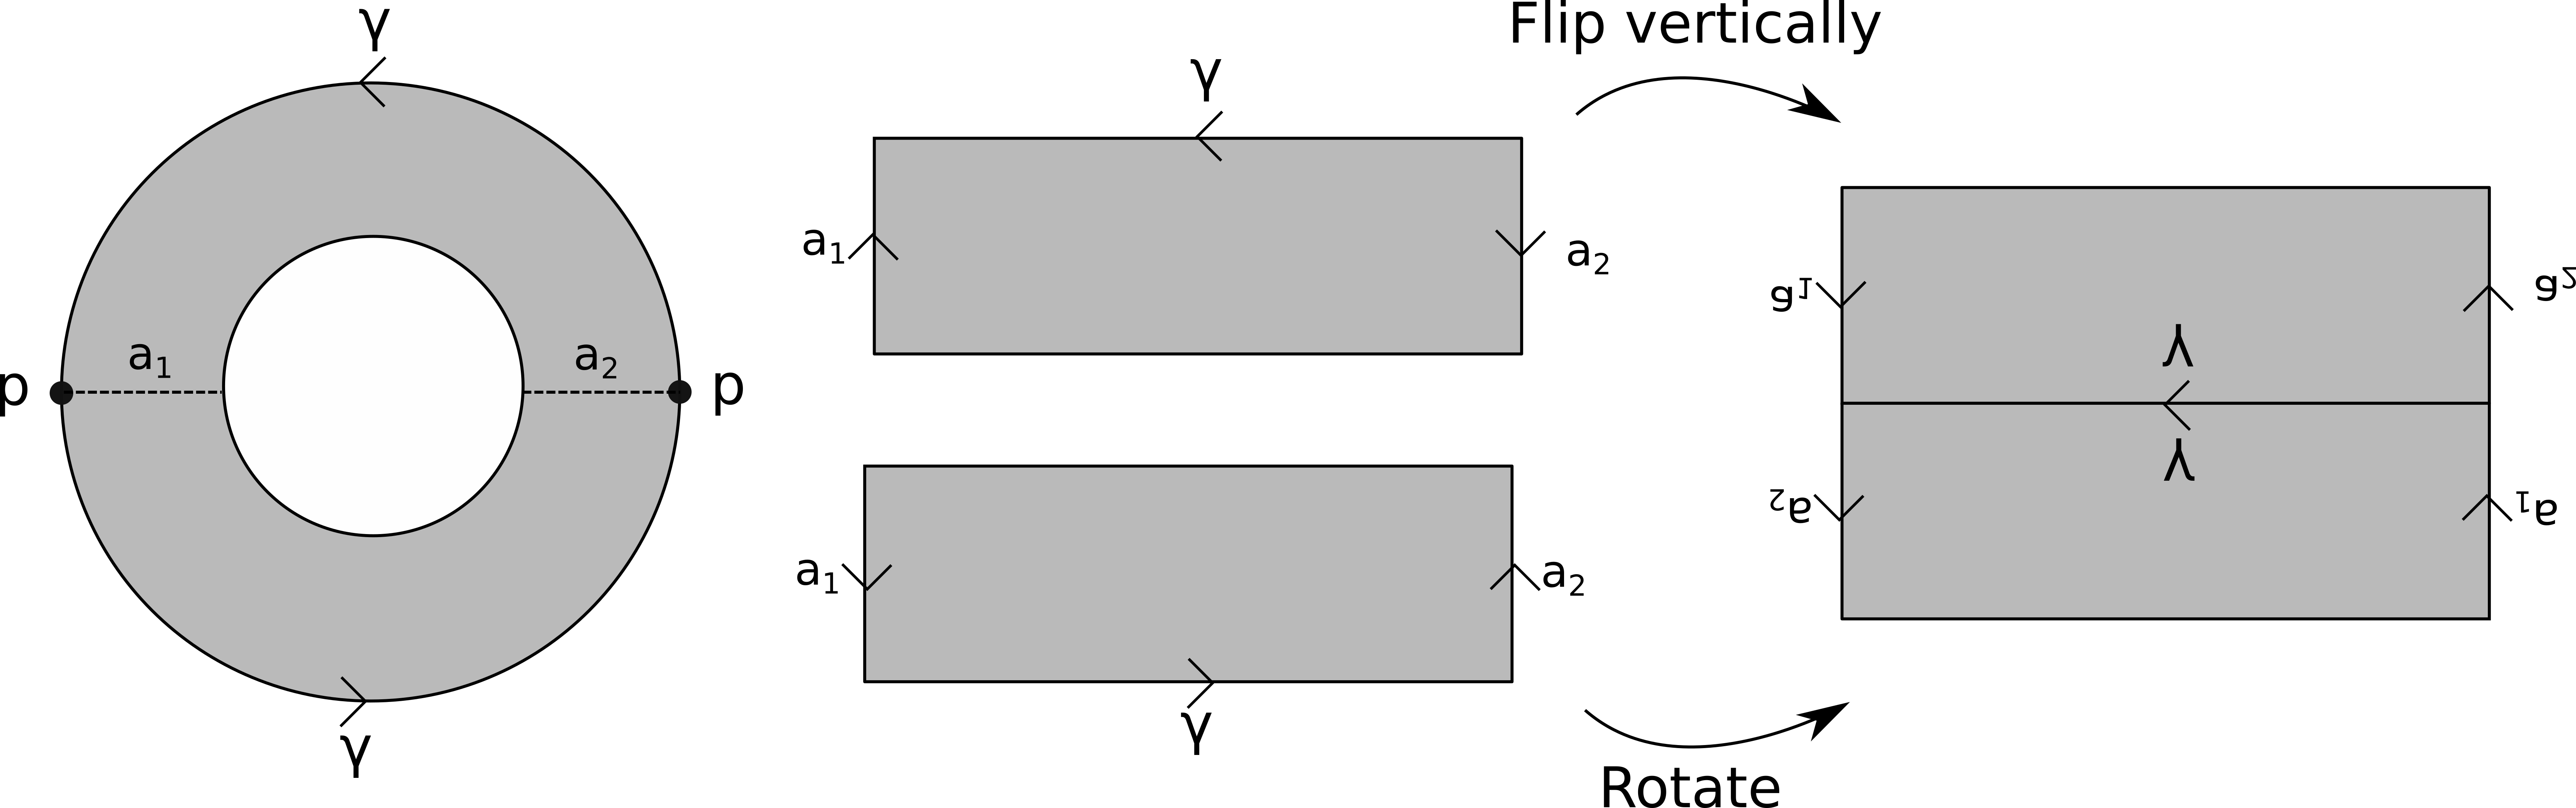
\includegraphics[width=5in]{rp2toM.png}
	\caption{Showing $X$ is homeomorphic to $M$}
	\label{fig:rp2toM}
\end{figure}

Denoting $a=a_1\ast a_2$ we recover the usual characterisation of the M\"obius strip.
Reversing this, we can in fact obtain the projective pain by glueing a 2-cell along the boundary of the M\"obius strip.

\subsubsection{Computing $\pi_1(\RP^2)$ from the M\"obius strip and S-vk}

\begin{figure}[ht]
	\centering
	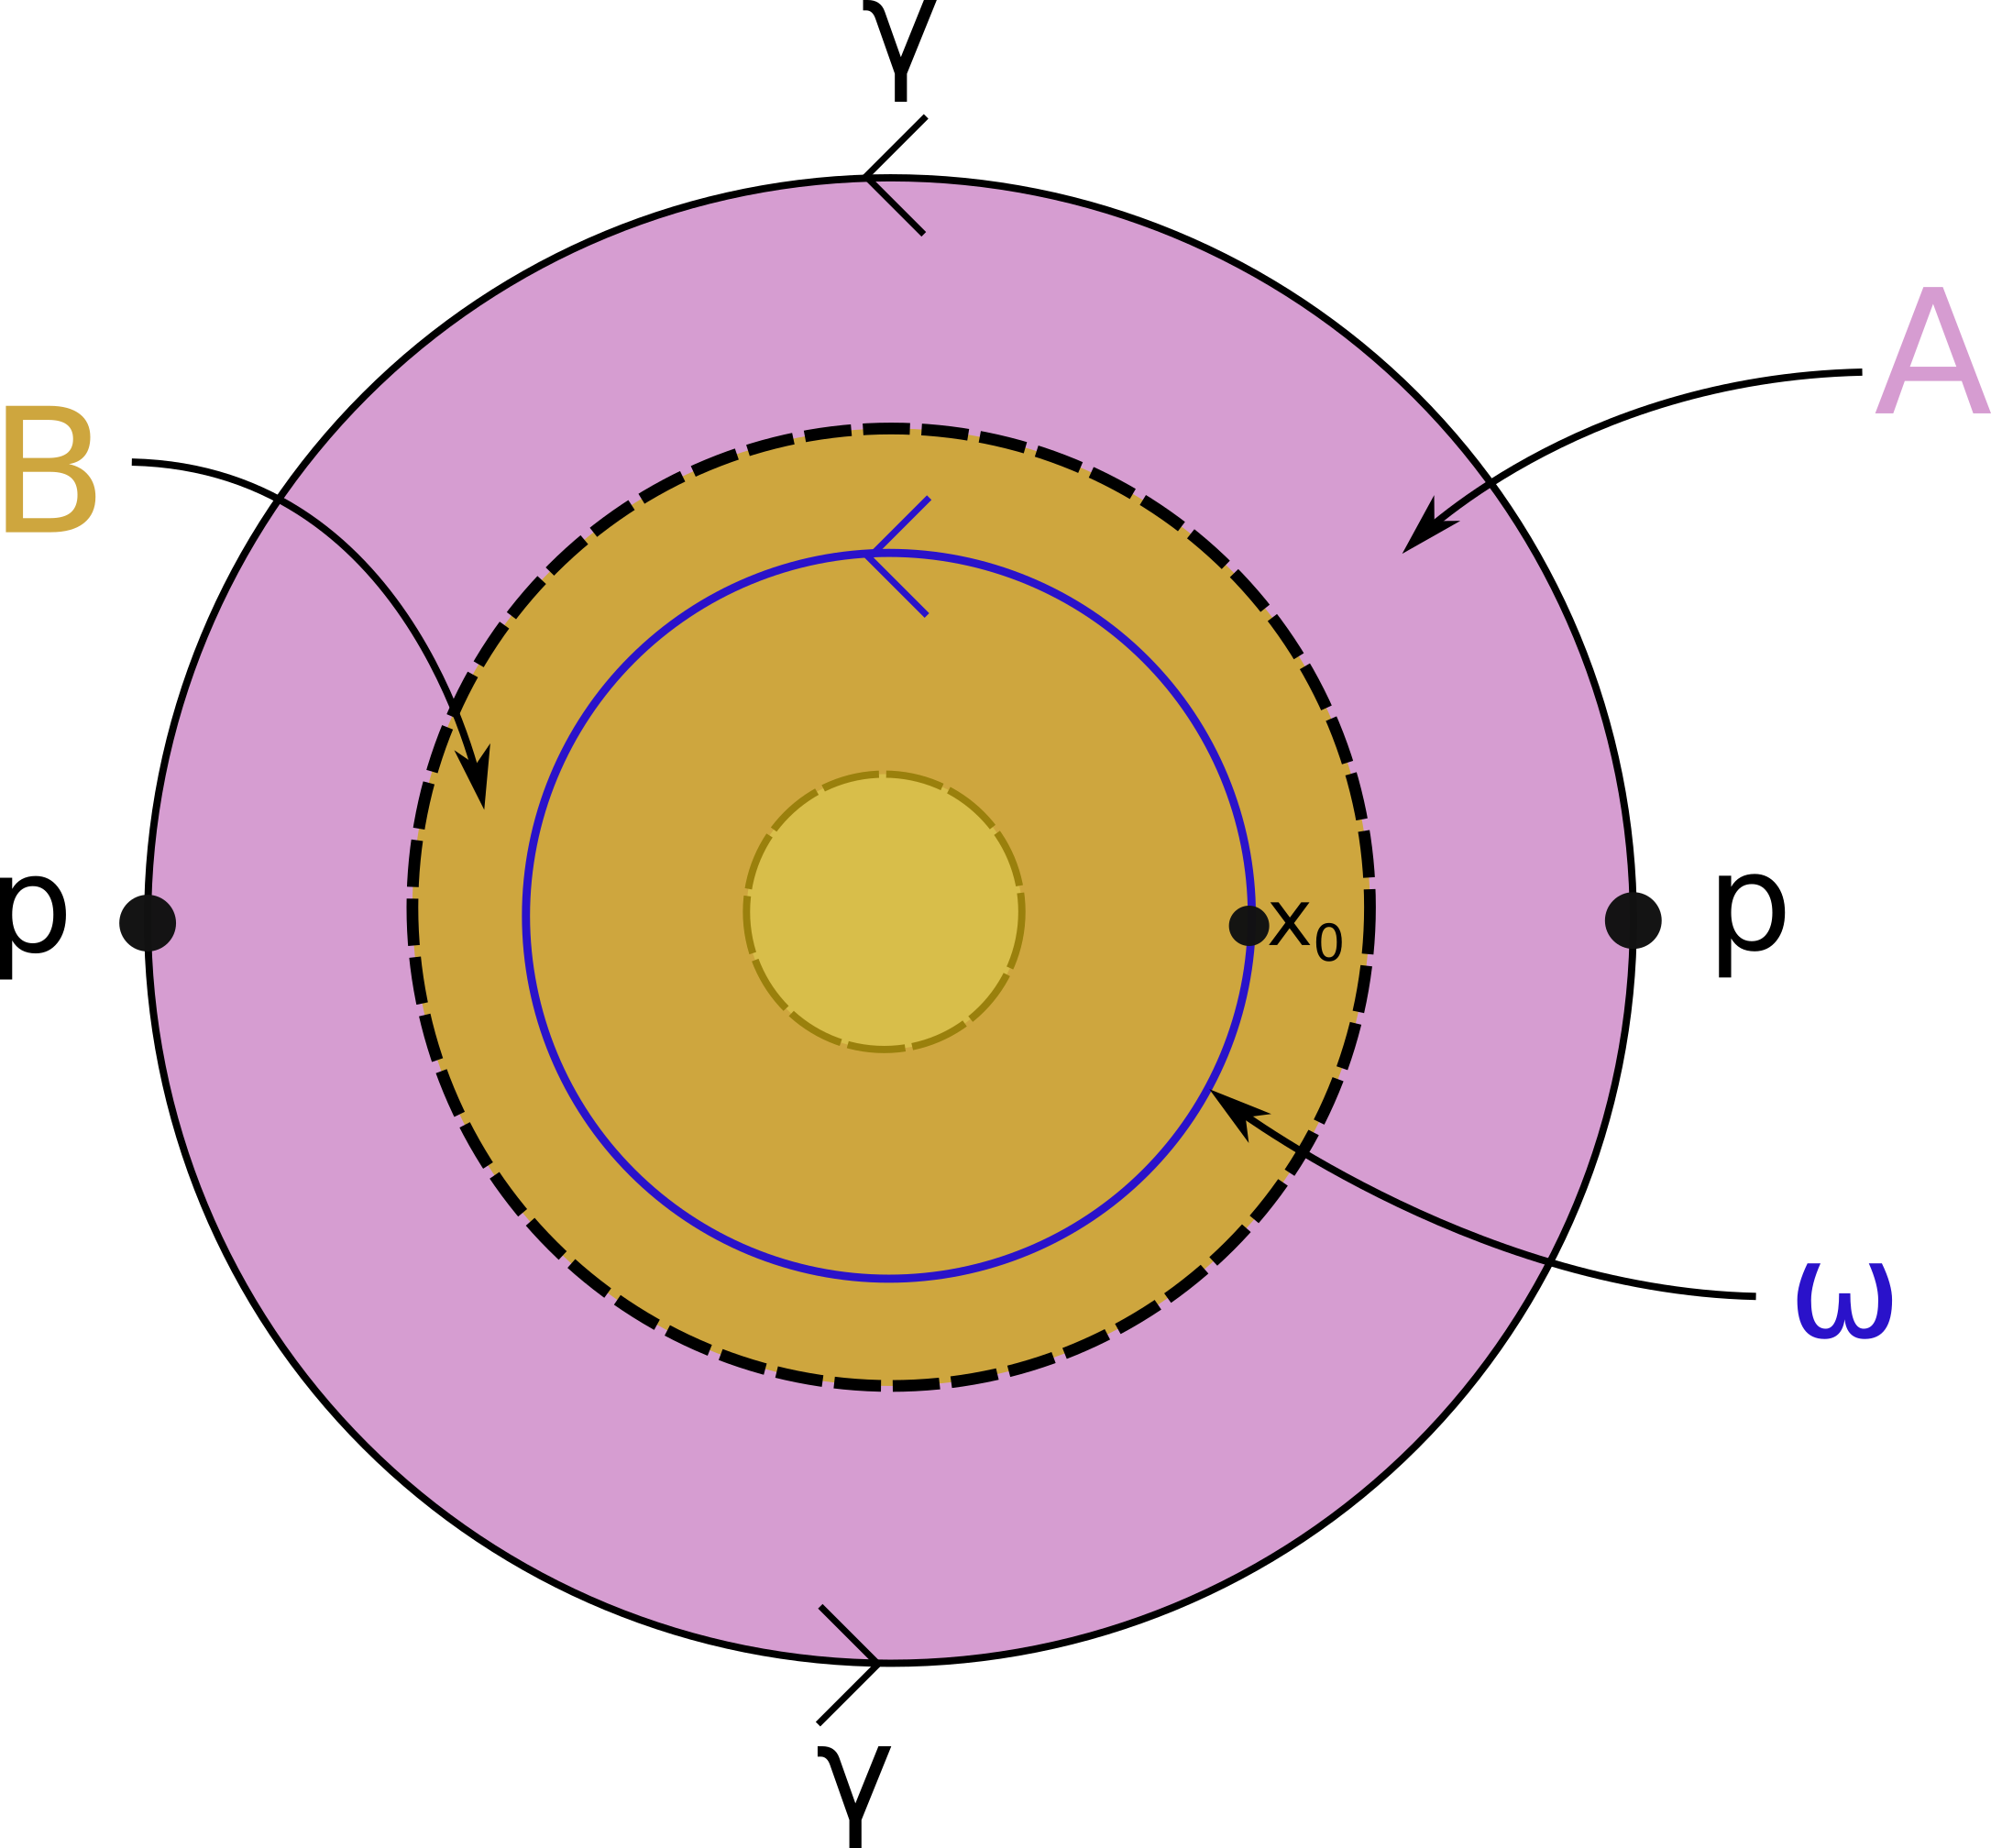
\includegraphics[width=3in]{rp2svk.png}
	\caption{Covering $\RP^2$ in order to compute $\pi_1$ by S-vK}
	\label{fig:rp2svk}
\end{figure}

We can use our previous construction of $\RP^2$ to create an open cover for $\RP^2$ by sets whose fundamental groups we understand.
Let $C$ be some small closed disc $C$ in the interior of the 2-cell and then take an open disc $B\supseteq C$.
Then define $A=\RP^2\setminus C$.

Now $A$ and $B$ form a cover for $\RP^2$, where $B$ is a disc and $A$ is the interior of a M\"obius strip.
Pick some $x_0\in A\cap B$.
Their intersection $A\cap B$ is an annulus which deformation retracts to a circle and hence $\pi_1(A\cap B, x_0)$ can be generated by a loop $\omega$ as shown in Figure \ref{fig:rp2svk}.

$A$ is the M\"obius strip and hence $\pi_1(A, x_0)=\langle\gamma\rangle\cong\Z$ the fundamental group is generated by the middle circle.
Finally $B$ is contractible and hence has trivial fundamental group.
The free group $\pi_1(A, x_0) \ast \pi_1(B, x_0)$ is generated by $\left[\gamma\right]$.
Since $B$ is trivial we only have to factor out multiplies of
\[
	(i_{A\cap B})_\ast(\left[\omega\right])
\]
where $i_{A\cap B}$ is the inclusion of $A\cap B$ in $A$.
Note $\omega$ is homotopic to the boundary circle of the M\"obius strip where as $\gamma$ is the inner circle.
Hence going round $\omega$ once is like going round $\gamma$ twice.
Consequently we have to factor out multiples of $\left[\gamma\right]^2$.
In conclusion,
\[
	\pi(\RP^2, x_0)\cong\frac{\langle\left[\gamma\right]\rangle}{\langle\left[\gamma\right]^2\rangle}\cong\frac{\Z}{2\Z}
\]

\subsection{Properties of CW complexes}
Given any $n$-cell $D_\alpha^n$ we construct the characteristic map as follows
\begin{figure}[H]
	\centering
	\begin{tikzcd}
		D_\alpha^n \arrow[r, hook, "i"] \arrow[rrr, bend left, "\Phi_\alpha^n"] & X^{n-1}\sqcup\bigsqcup_\alpha D_\alpha^n \arrow[r, "q"] & X^n \arrow[r, hook] & X
	\end{tikzcd}
\end{figure}

Recall that a \mdf{subcomplex} is a space $A$ that is a union of cells $e_\alpha^n$ in $X$ such that for every cell it also contains its closure in $X$.
\begin{prop}
A compact topological subspace of a CW complex $X$ is contained in a finite subcomplex.
\end{prop}
\begin{proof}
Might be worth reading this.
\end{proof}
\begin{defin}
The C is in CW complex stands for \mdf{closure finiteness} meaning that the closure of every open cells meets only finitely many other cells.
The W stands for weak topology.

A topological space is called
\begin{itemize}
	\item \mdf{normal} if any two disjoint closed subsets have disjoint open neighbourhoods.
	\item \mdf{Hausdorff} if any two distinct point have disjoint open neighbourhoods.
	\item \mdf{locally contractible} if around every point $x$ and neighbourhood $x\in U \subseteq X$ there is an open $V$ with $x\in V \subseteq U $ such that $V$ is contractible.
\end{itemize}
\end{defin}

\begin{eg}
The Warsaw circle is not locally contractible
\[
	W=\left\{(c, \sin(1/x) \rmv x \in (0, 1] \right\}\cup \left(\left\{0\right\}\times [-1, 1]\right)\cup L
\]
where $L$ is a curve joining the first set to the second set, with the subspace topology.
\end{eg}

\begin{prop}
CW complexes are locally contractible.
\end{prop}

\begin{prop}
\label{prop:subdr}
If $A\subseteq X$ is a subcomplex of a CW complex $X$ then there exists an open set $U\subseteq X$  with $A\subseteq U$ such that $U$ deformation retracts to $A$.
\end{prop}

An important application is that we can decompose CW complexes $A$ and $B$ such that $A\cap B$ is a subcomplex and then use Seifert-can Kampen.
One can use the above proposition to show that the fundamental group of a CW complex depends only on the 2-skeleton.
However we will give a proof using the Seifert-van Kampen Theorem.

We begin with the following observation.
Suppose $X$ is a topological space and $\phi_\alpha:S^1_\alpha \to X$ is a map that attaches a 2-cell $D_\alpha^2$ to $X$ then $\phi_\alpha$ defines a loop $f_\alpha:I \to X$ in $X$ which is based at $\phi_\alpha(1)$.
This loop may not be null-homotopic in $X$ but it certainly is after we attach $D_\alpha^2$, namely in the space
\[
	Y\defeq X\sqcup\frac{D_\alpha^2}{x\sim\phi_\alpha(x)}
\]
If $X$ is path-connected then we can choose a base point $x_0\in X$ and a path $h_\alpha:I \to X$ from $x_0$ to $\phi_\alpha(1)$ and then we get a loop
\[
	\gamma_\alpha\defeq h_\alpha \ast f_\alpha \ast \overline{h_\alpha}
\]
In this way, every attaching map gives us a loop in Y.
Note that the inclusion map $X \hookrightarrow Y$ induces a map of fundamental groups $\pi_1(X, X_0)\to\pi_1(Y, y_0)$ under which the class of every such loop, $\left[\gamma_\alpha\right]$ is sent to $0$ because these loops are contractible in $Y$.

\begin{prop}
Let $X$ be a path-connected topological space and for some fixed $N$ let $\phi_\alpha^N:S_\alpha^{n-1}\to X$ be some collection of attaching maps.
Set
\[
	Y\defeq X\sqcup\bigsqcup_\alpha\frac{D_\alpha^n}{x\sim \phi_\alpha^n (X)}
\]
Let $x_0\in X$ be a point.
Then
\begin{itemize}
	\item If $n=2$, then
		\[
			\pi_1(Y, x_0)\cong \faktor{\pi_1(X,x_0)}{N}
		\]
		where $N$ is the normal subgroup generated by the element $\left[\gamma_\alpha\right]$ as defined previously.
	\item If $n>2$, then
		\[
			\pi(Y, x_0)\cong \pi_1(X, x_0)
		\]
\end{itemize}
\end{prop}

\begin{proof}
There is a sketch proof in the notes that may be worth reading.
\end{proof}

\begin{theorem}
For a path-connected CW-complex $X$ with $x_0\in X^2$, the inclusion map $X^2\hookrightarrow X$ induces an isomorphism of fundamental groups $\pi_1(X^2, x_0)\cong \pi_1(X, x_0)$.
\end{theorem}

\begin{proof}
This follows automatically from the previous proposition of $X$ is finite dimensional because it tells us that the fundamental group does not change when we add an $n$-cell where $n>2$.

If $X$ is not finite-dimensional then note that a loop $\gamma$ in $X$ is a compact subset and therefore contained in a finite subcomplex in some $X^n$. Since $\pi_1(X^2, x_0)\cong \pi_1(X^n, x_0)$ every such loop is homotopic to a loop in $X^2$ and therefore the map $\pi_1(X^2, x_0)\to \pi(X, x_0)$ is surjective.

To see that it is injective, let $\gamma$ be a loop in $X^2$ such that it is homotopic, in $X$, to the constant loop via some homotopy $F:I\times I \to X$.
The image of $F$ in $X$ is compact and hence contained in a finite subcomplex $X^n$ and we can safely assume that $n>2$.
It follows therefore that $\left[\gamma\right]=0$ in $\pi_1(X^n, x_0)$.
Then $\pi_1(X^2, x_0)\to\pi_1(X^n, x_0)$ is injective and hence $\gamma$ is null-homotopic in $X^2$.
\end{proof}

We can also prove this with Proposition \ref{prop:subdr}.
For a proof of this consult Lecture 26.

\subsection{Generators and Relations}

When using the Seifert-van Kampen theorem we often obtain a presentation of a group in terms of a group quotient some normal subgroup.
When these groups are finitely generated it is natural to present this group as a number of generators and relations.


\begin{figure}[ht]
	\centering
	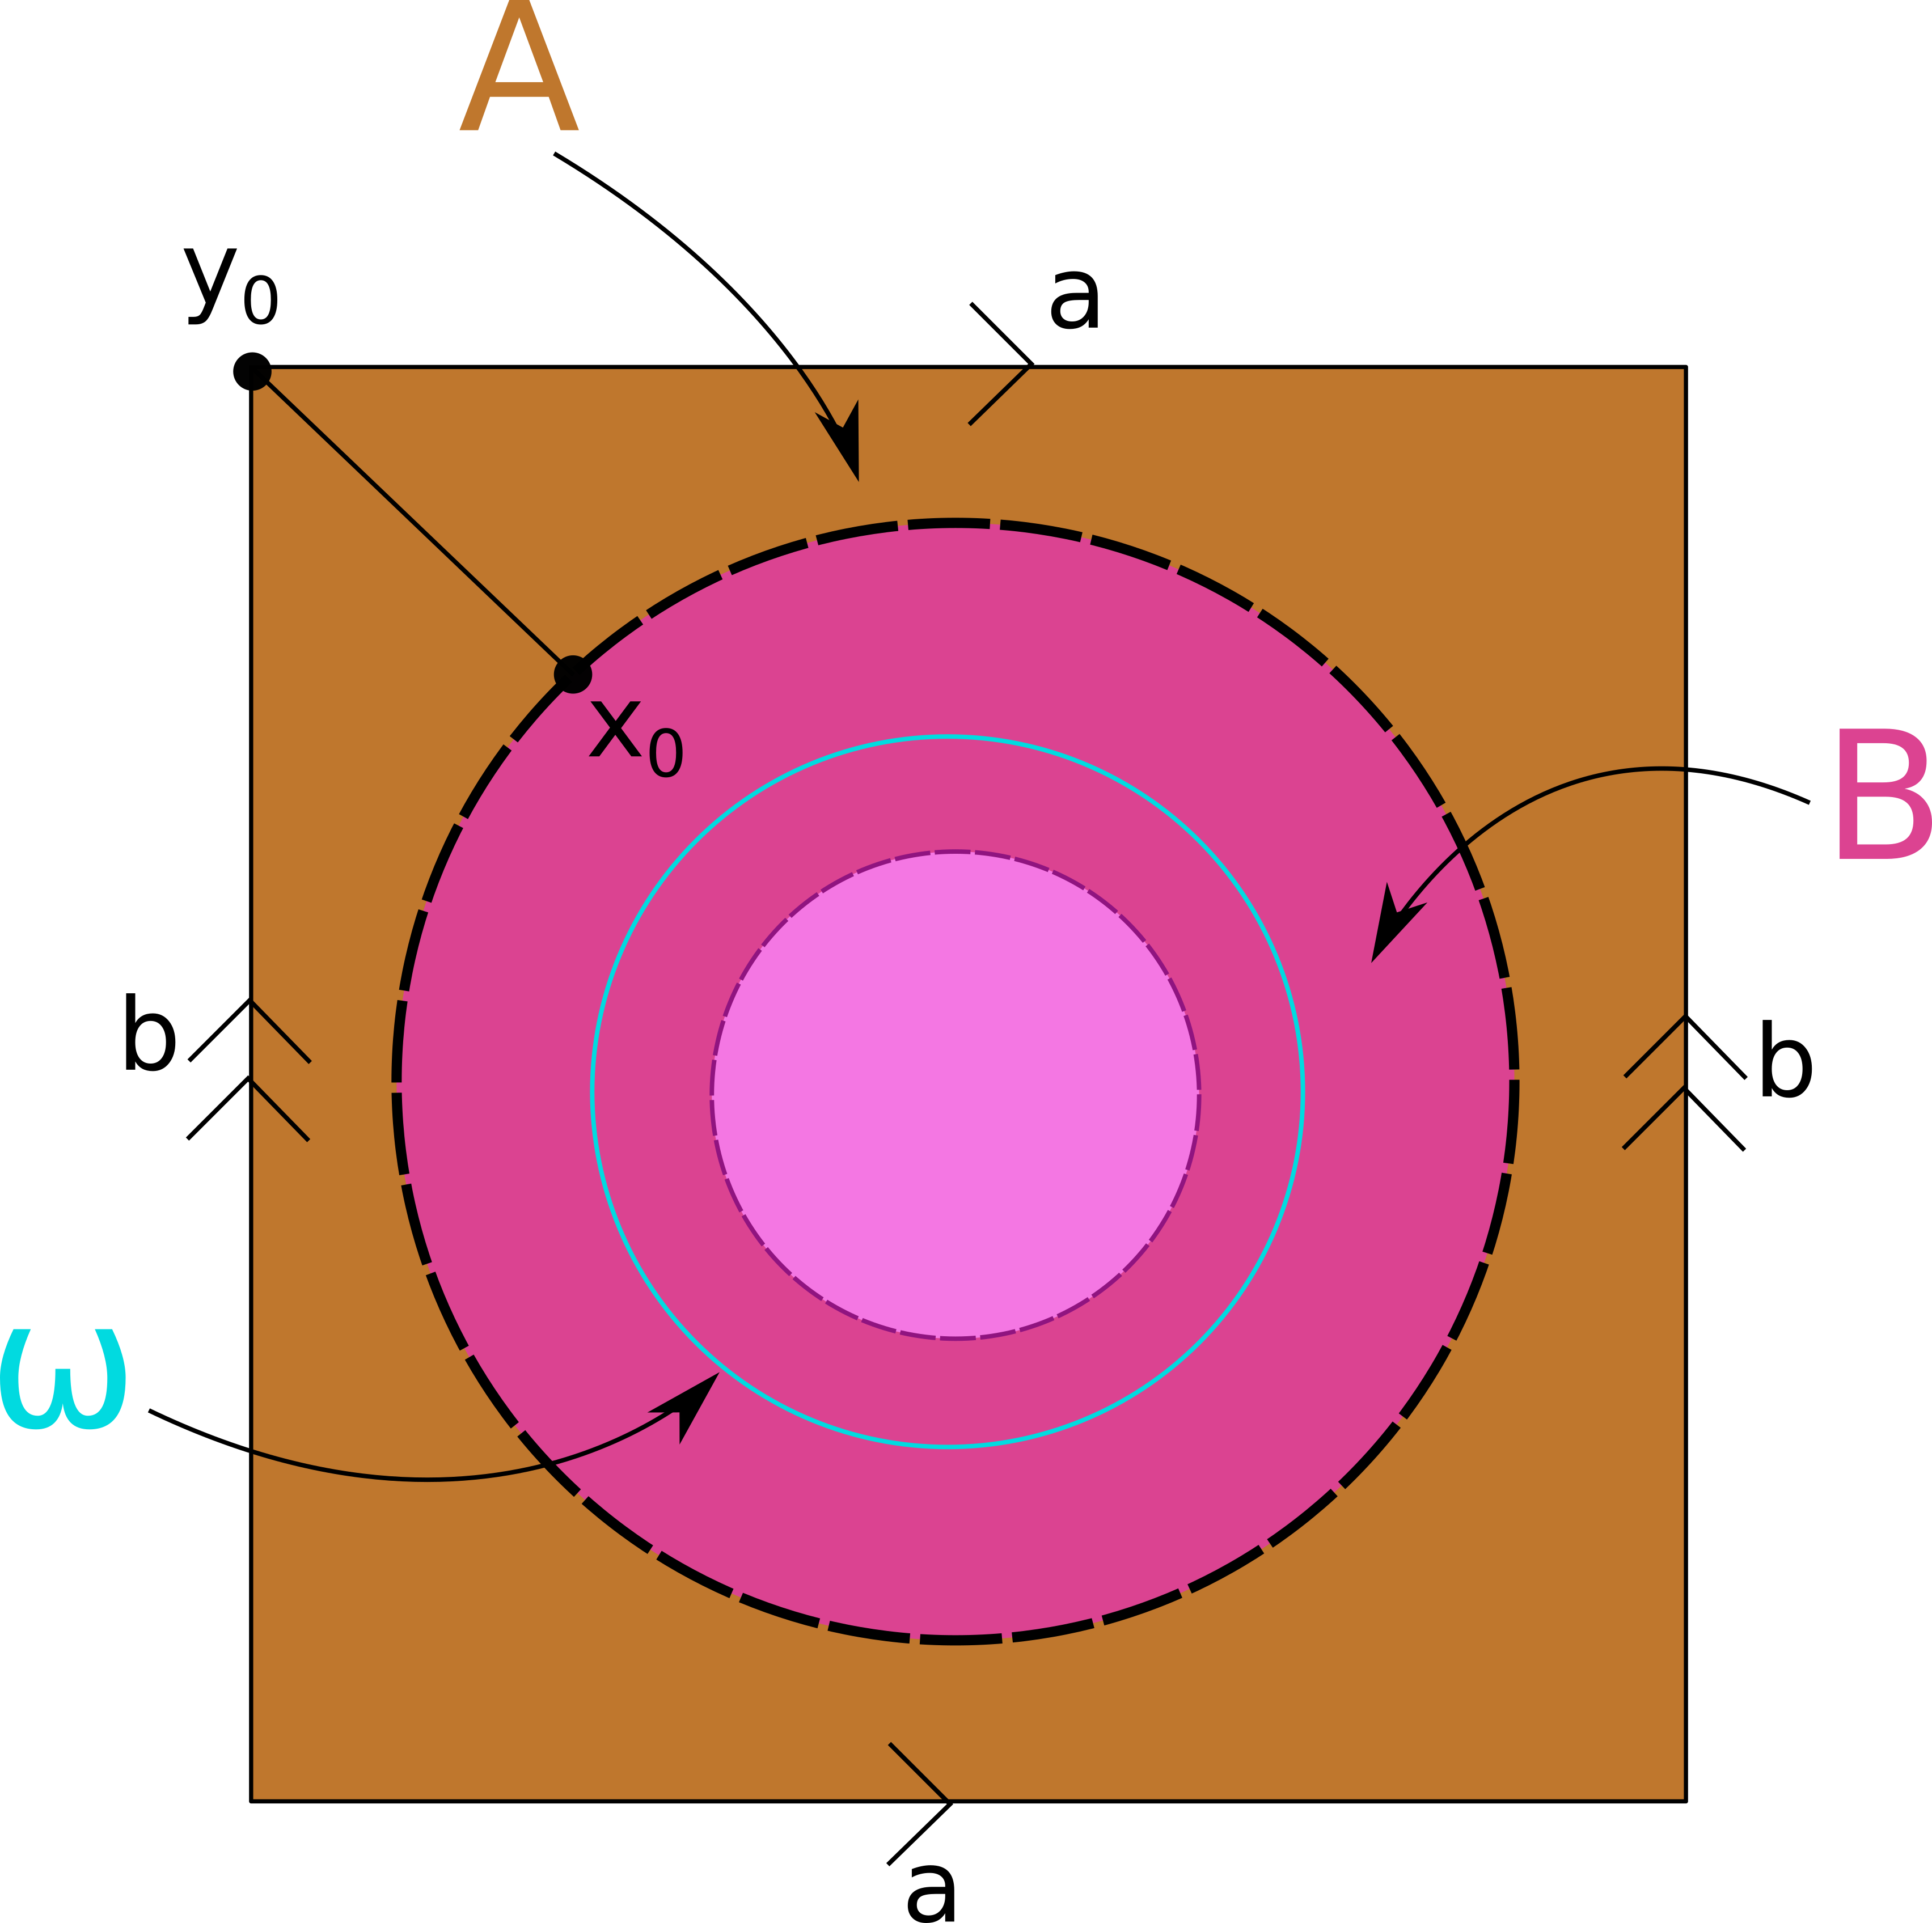
\includegraphics[width=3in]{torussvk.png}
	\caption{Computing the fundamental group of $\mathbb{T}^2$ by S-vK}
	\label{fig:torussvk}
\end{figure}

For example, consider the decomposition of the torus shown in Figure \ref{fig:torussvk}.
We see that $A$ deformation retracts to a wedge sum of two circles with generators $[a]$ and $[b]$.
Then $B$ is contractible and so makes no contribution to the final fundamental group.
So $\pi_1(\mathbb{T}^2)$ will be some quotient of $\langle\left[a\right]\rangle\ast\langle\left[b\right]\rangle$.

Finally $A\cap B$ is homotopy equivalent to $S^1$ and is hence generated by some inner loop $\omega$.
We need to quotient out by the normal subgroup generated by $\left(i_{AB}\right)_\ast([\omega])$.
One can see that in $A$ the loop $\omega$ is, up to homotopy, equal to $aba^{-1}b^{-1}$.
Hence the fundamental group is presented as
\[
	\pi_1(\mathbb{T}^2)=\frac{\langle\left[a\right]\rangle\ast\langle\left[b\right]\rangle}{\langle\langle aba^{-1}b^{-1}\rangle\rangle}
\]
We say $\left[a\right]$ and $\left[b\right]$ are \mdf{generators} and $\left[aba^{-1}b^{-1}\right]$ is a \mdf{relation}.
We say that his relation is equivalent to making the group abelian and hence
\[
	\pi_1(\mathbb{T}^2)\cong\Z\times \Z
\]
\begin{note}
This technique can be used to calculate the fundamental group of the surface of genus $g$.
We can create the surface by taking a $4g$-gon and quotient sides by the sequence
\[
	a_1, b_1, a_1^{-1}, b_1^{-1}, a_2, b_2, a_2^{-1}, b_2^{-1}, \dots, a_n, b_n, a_n^{-1}, b_n^{-1}
\]
Then poking a hole in the middle yields a surface which deformation retracts to a wedge of $2g$ circles.
So we start with $2g$ generators $a_1, b_1, \dots, a_n, b_n$ and then our relation is just the sequence describing boundary of the $4g$-gon.
\end{note}

\begin{defin}
	A group $G$ is a \mdf{presentation} as
	\[
		\langle S | R\rangle,
	\]
	where $S$ is a set of \mdf{generators} and $R$ is a set of \mdf{relators} if $G$ is the free group generated by the elements of $S$ modulo the normal subgroup generated by $R$, i.e.
	\[
		G=\faktor{\langle S\rangle}{\langle\langle R\rangle\rangle}
	\]
	A group is called \mdf{finitely generated} if it has a finite set $S$ of generators and \mdf{finitely presented} if both $S$ and $R$ are finite sets.
\end{defin}

\subsection{Computing the fundamental group}
From what we have seen we can make the following simplifications to compute $\pi_1$ of some CW complex $X$ at $x_0\in X$:
\begin{itemize}
	\item We may assume $X$ is path connected because the fundamental group at $x_0$ only concerns the path-component of $x_0$.
	\item $X=X^2$ because the fundamental group can only discern the structure of a CW complex up to the 2-skeleton.
	\item $x_0\in X^1$ because $X$ is path connected so the fundamental group will not change.
\end{itemize}

To compute the fundamental group of $X$ we proceed as follows:

\begin{enumerate}
	\item Find a spanning tree $T\subseteq X^1$.
		Let $\mathcal{A}$ denote the set of edges not in the tree.
		Pasting any such edge into $T$ gives a subgraph that is homotopic to $S^1$ (an edge-cycle).
		We have seen in exercises that we can then describe the fundamental group of the 1-skeleton as
		\[
			\pi_1(X^1, x_0)\cong \bigast_{e\in\mathcal{A}}\Z.
		\]
		Every edge not in $T$ yields a loop when added to $T$ and conversely every loop in $X^1$ based at $x_0$ is homotopic to a combination of edge-cycles which are loop which consist of traversing some cycle which arose by adding $a\in\mathcal{A}$.
	\item Let $e_\alpha^2\subseteq X^2$ be some 2-cell and let $\phi_\alpha : S_\alpha^1\to X^1$ be the attaching map.
		Note that looping once around the boundary where we attach $e_\alpha^2$ yields a loop in $X^1$.
		Hence after adjoining connecting paths to $x_0$ we obtain a loop based at $x_0$ which corresponds to a reduced word $u_\alpha$ in $\pi_1(X^1, x_0)$.
		Let $U\defeq\left\{U_\alpha\right\}_\alpha$ denote the set of all such words.

		\textbf{Claim: }We can now compute the fundamental group as
		\[
			\pi_1(X, x_0)\cong\faktor{\pi_1(X^1, x_0)}{\langle\langle U\rangle\rangle}
		\]
		or more concisely, the fundamental group can be presented as $\langle\mathcal{A} | U \rangle$.
\end{enumerate}

\begin{proof}
\begin{itemize}
	\item The union of all the cells $e_\alpha^2$ together with paths joining them to $x_0$ form a contractible subcomplex $A$ so
		\[
			\pi_1(A, x_0)\cong 1
		\]
	\item Choose points $y_\alpha\in e_\alpha^2$ inside each of the cells and define a new subset
		\[
			B\defeq X^2 \setminus \bigcup_\alpha\left\{y _\alpha\right\}.
		\]
		Then $B$ retracts to the 1-skeleton $X^1$ because we have "poked a hole" into each of the 2-cells.
		Hence $\pi_1(B, x_0)\cong \pi_1(X^1, x_0)$.
	\item We can write $X^2 = A\cup B$ and now $A\cap B$ deformation retracts to a graph consisting of cycles starting at $x_0$ such that the boundary of every 2-cell is homotopic to some cycle in $A \cap B$ starting at $x_0$.
		In other words, each element of $\pi_1(A\cap B, x_0)$ represents a word in $U$.
	\item By Seifert-van Kampen we therefore have that the fundamental group of $X$ is given by
		\[
			\pi_1(X, x_0)\cong\faktor{\pi_1(A, x_0)\ast\pi_1(B, x_0)}{\langle\langle U\rangle\rangle}\cong\faktor{\pi_1(X^1, x_0)}{\langle\langle U\rangle\rangle}
		\]
\end{itemize}
\end{proof}

\begin{figure}[ht]
	\centering
	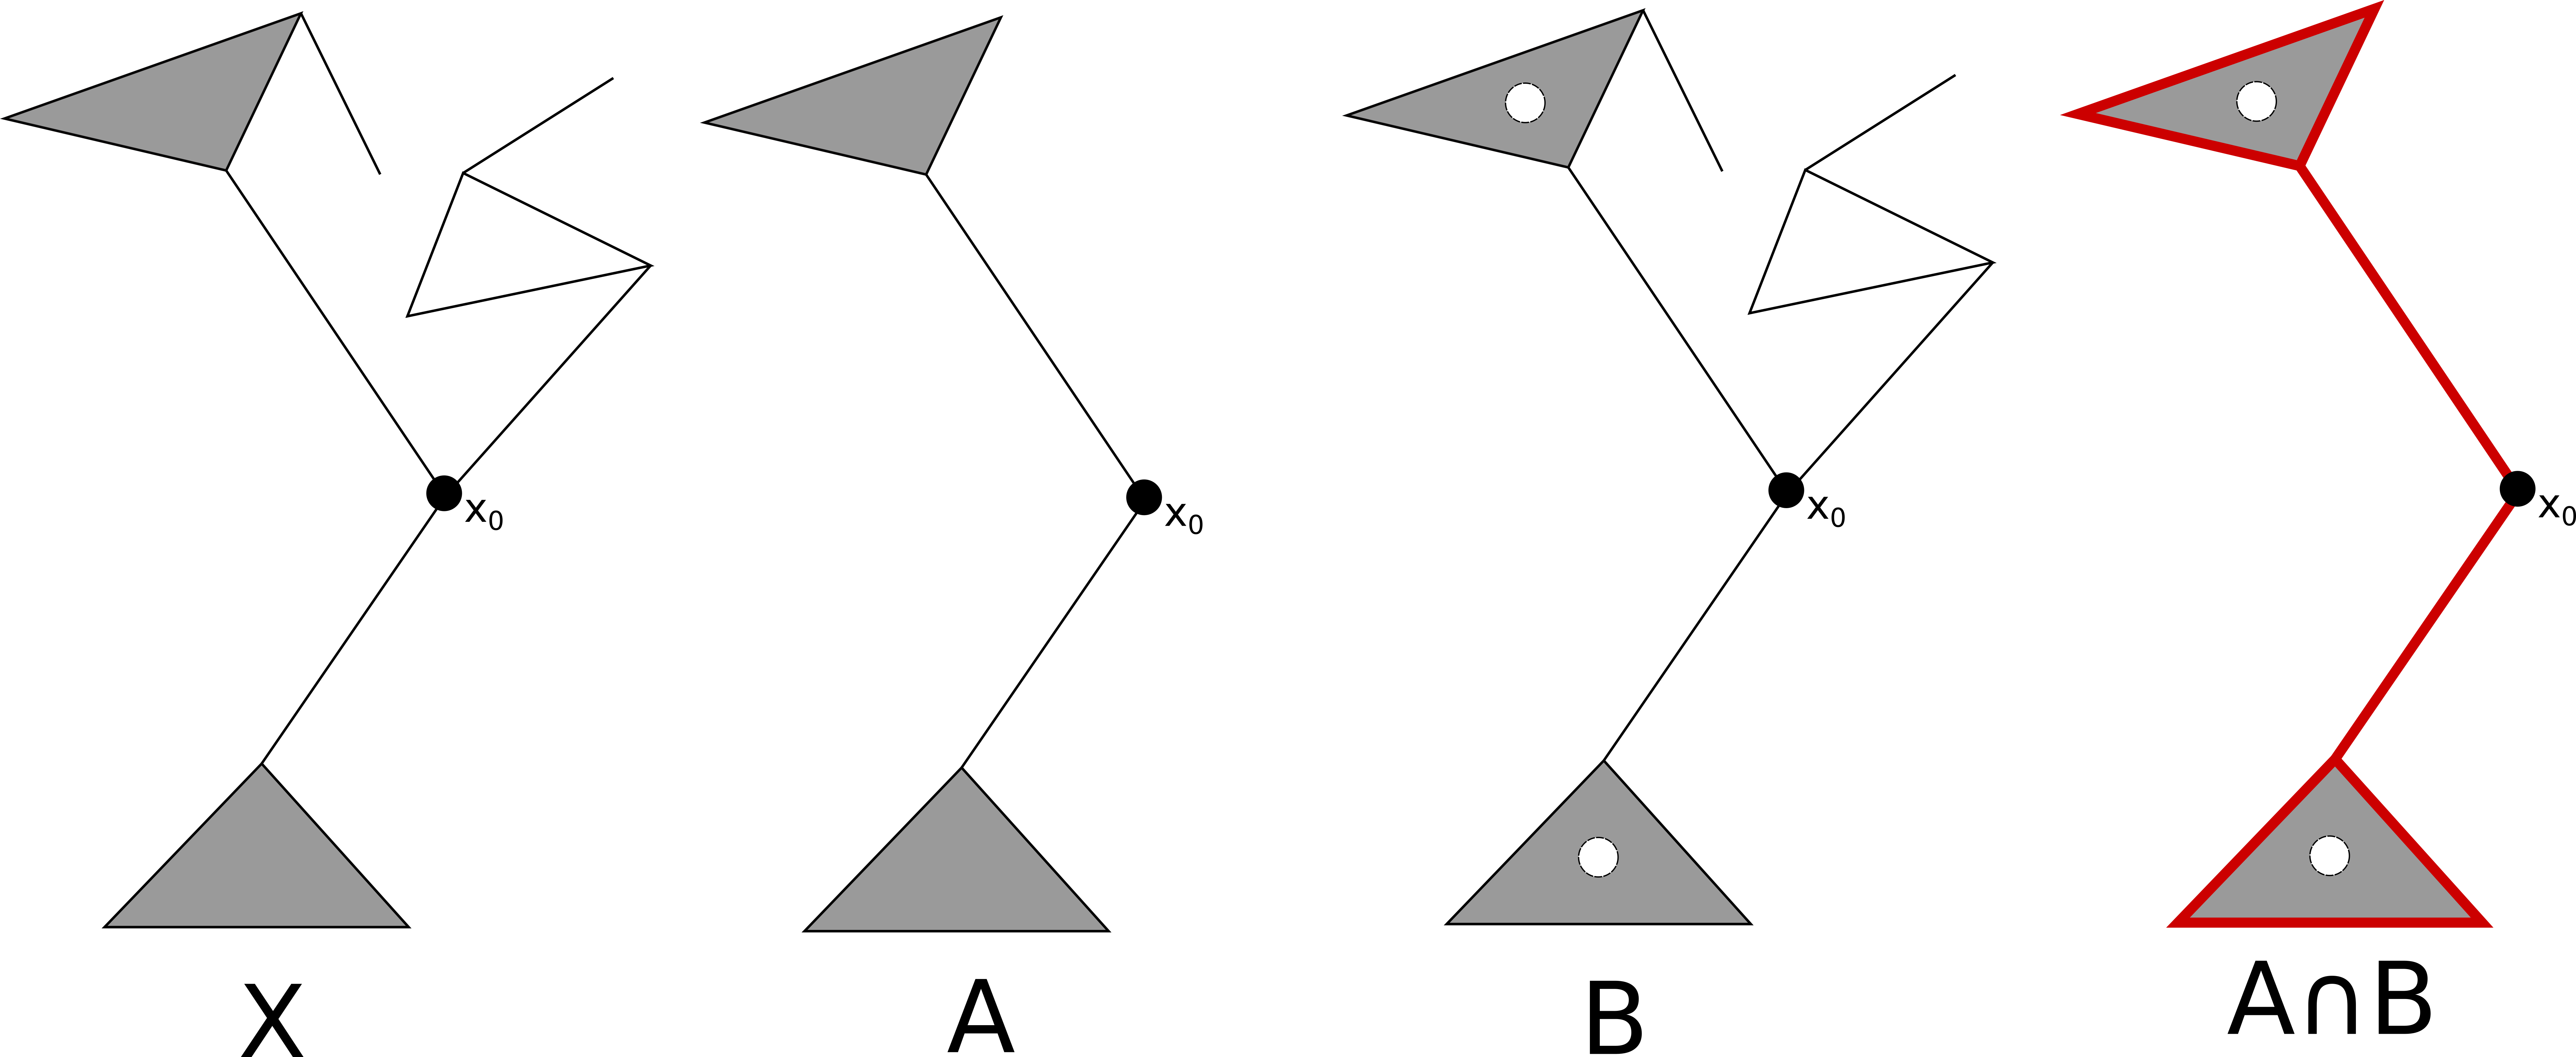
\includegraphics[width=5in]{CWpi1.png}
	\caption{An example of the construction of $A$ and $B$, red paths indicated the relators in $U$}
\end{figure}

In summary

\begin{itemize}
	\item Every \mdf{cycle} in the underlying $X^1$ corresponds to a loop based at $x_0$ which moves from $x_0$ to the cycle, goes around the cycle and then reutrns.
		Every such cycle corresponds to a \mdf{generator} of the fundamental group $\pi_1(X^2, x_0)$.
	\item Every \mdf{loop} in $X^2$ can be represented as a combination of such loops.
		This correspodns to a reduced \mdf{word} in the generators of $\pi_1(X^2, x_0)$.
	\item A loop is \mdf{null-homotopic} if it is homotopic to the boundary of a 2-cell in $X^2$.
		Such loops correspond to a \mdf{relation} on the set of words in $\pi_1(X^2, x_0)$.
\end{itemize}

There are number of useful examples of how this process is used in the final lecture notes.
Finally, we have a converse theorem that says that every group arises as the fundamental group of some space.

\begin{theorem}
For every group $G$ there exists a path-connected two-dimensional CW complex $X_G$ such that
\[
	\pi_1(X_G)\cong G
\]
\end{theorem}

\begin{proof}
Consider a presentation of the group with generators and relators.
Construct the one skeleton $X^1$ as a wedge of circles $S^1$, one per generators.
Every relater then describes a loop in $X^1$.
For each such relator, take a 2-cell $D_\alpha^2$ with boundary $S_\alpha^1$ and define attaching map that maps the circle onto the loop specified by the relators.
\end{proof}

\end{document}
